% LTeX: language=fr
%%%%%%%%%%%%%%%%%%%%%%%%%%%%%%%%%%%%%%%%%%%%%%%%%%%%%%%%%%%%%%%%%%%%%%%%%%
%%%%%                         CHAPITRE 3                            %%%%%%
%%%%%%%%%%%%%%%%%%%%%%%%%%%%%%%%%%%%%%%%%%%%%%%%%%%%%%%%%%%%%%%%%%%%%%%%%%

\lhead[\fancyplain{}{\leftmark}]%Pour les pages paires \bfseries
      {\fancyplain{}{}} %Pour les pages impaires
\chead[\fancyplain{}{}]%
      {\fancyplain{}{}}
\rhead[\fancyplain{}{}]%Pour les pages paires 
      {\fancyplain{}{\rightmark}}%Pour les pages impaires \bfseries
\lfoot[\fancyplain{}{}]%
      {\fancyplain{}{}}
\cfoot[\fancyplain{}{\thepage}]%\bfseries
      {\fancyplain{}{\thepage}} %\bfseries
\rfoot[\fancyplain{}{}]%
     {\fancyplain{}{\scriptsize}}
     
%/!\/!\/!\/!\/!\/!\/!\/!\/!\/!\/!\/!\/!\/!\/!\/!\/!\/!\/!\/!\/!\/!\/!\/!\ SECTION
    %///////////////////////////////////////////// sous-section
    		%************* sous-sous-section
    					 %--------- paragraphe
    					 
%%%%%%%%%%%%%%%%%%%%%%%%%%%%%%%%%%%%%%%%%%%%%%%%%%%%%%%%%%%%%%%%%%%%%%%%%%
%%%%%                      Start part here                          %%%%%%
%%%%%%%%%%%%%%%%%%%%%%%%%%%%%%%%%%%%%%%%%%%%%%%%%%%%%%%%%%%%%%%%%%%%%%%%%%
%%%%%%%%%%%%%%%%%%%%%%%%%%%%%%%%%%
%\begin{figure}[!htbp]
%\begin{center}
%    \captionsetup{justification=centering}
%	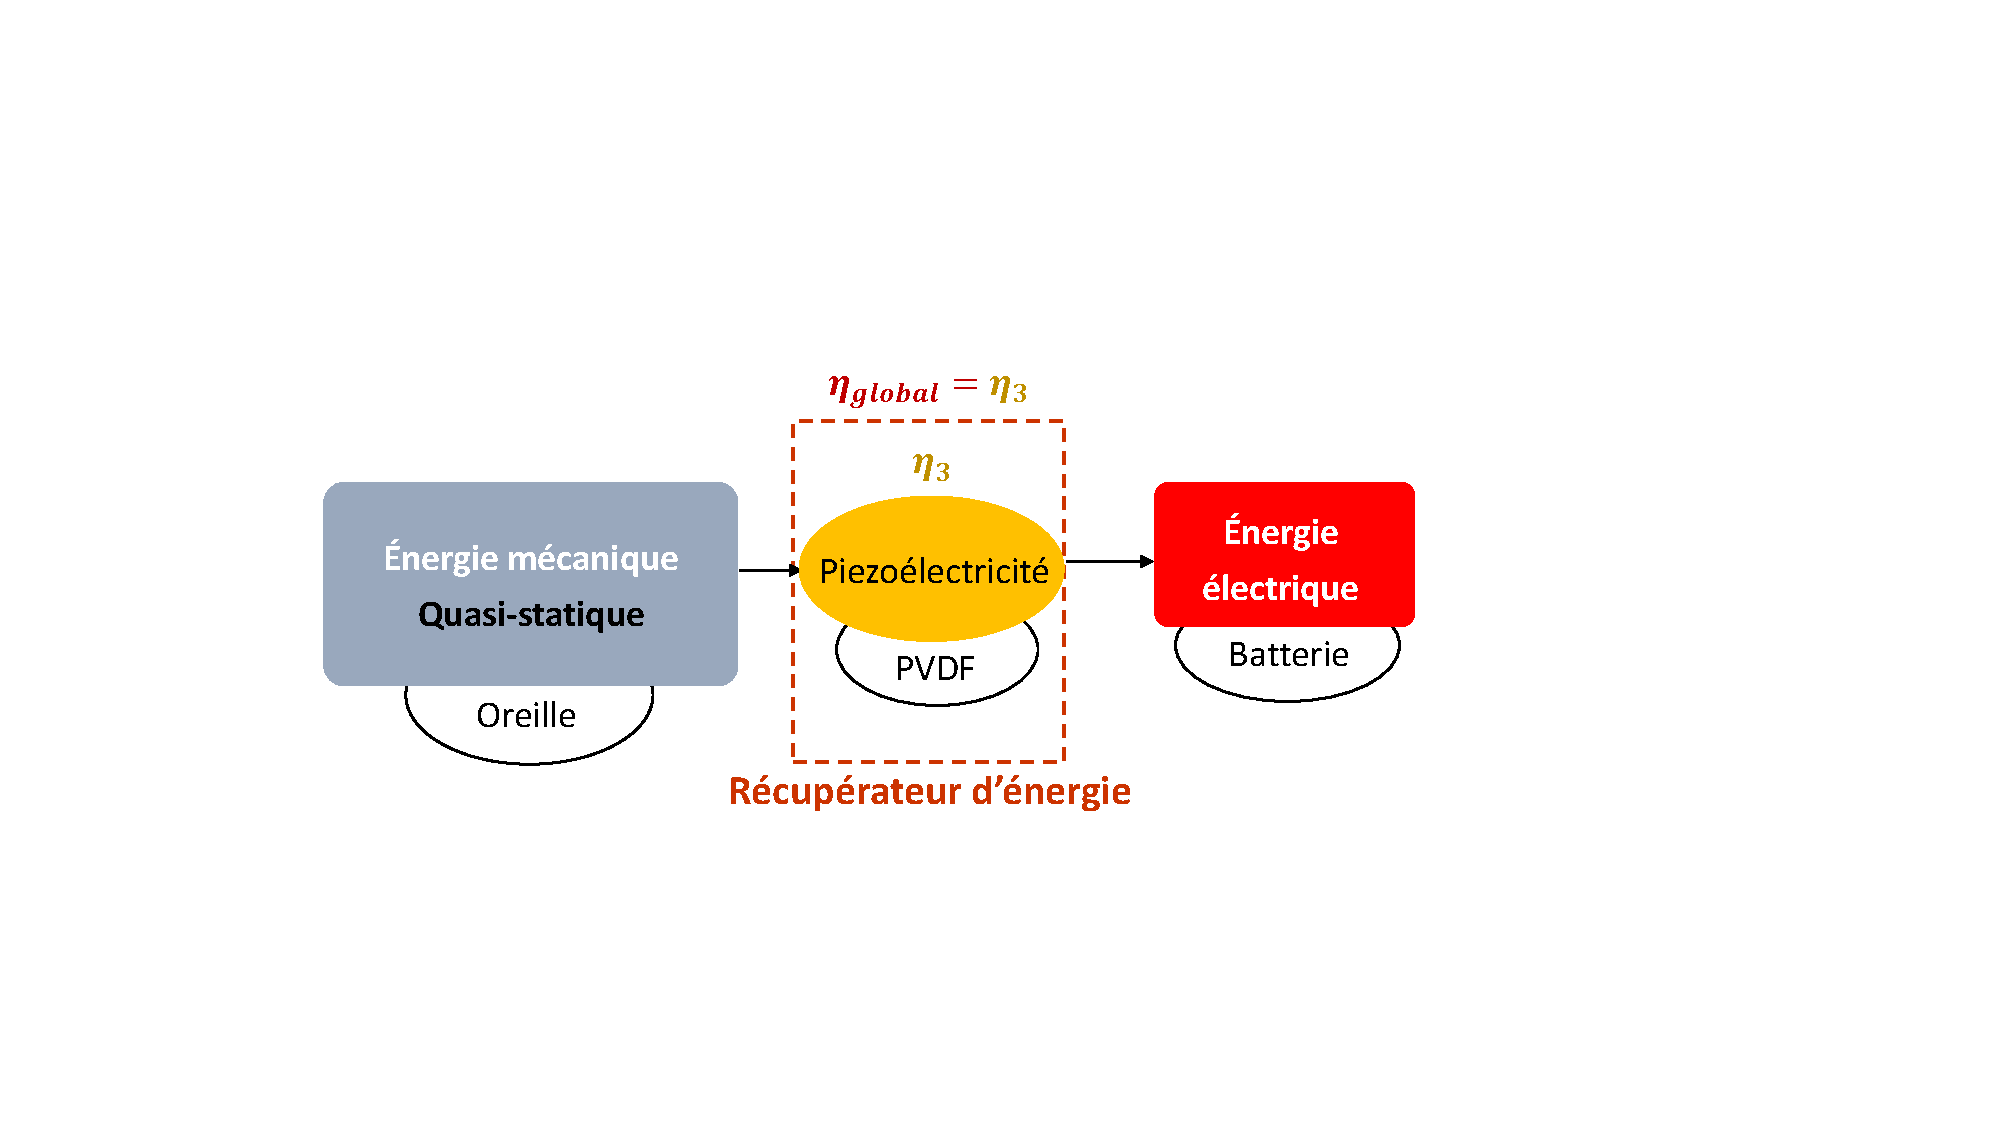
\includegraphics[trim={5cm 5cm 7cm 6cm},clip, width=0.7\textwidth]{../Chap3/Figure/conversion_critias_pvdf.pdf}
%	\caption{Chaîne de conversion énergétique pour la solution électromagnétique de Delnavaz \& Voix \cite{Delnavaz2013}}
%	\label{fig:conversion_critias_pvdf}
%\end{center}
%\end{figure}
%%%%%%%%%%%%%%%%%%%%%%%%%%%%%%%%%%
%%%%%%%%%%%%%%%%%%%%%%%%%%
%\begin{figure}[!htbp]
%\begin{center}
%	\begin{subfigure}[b]{0.45\textwidth}
%    \captionsetup{justification=centering}
%	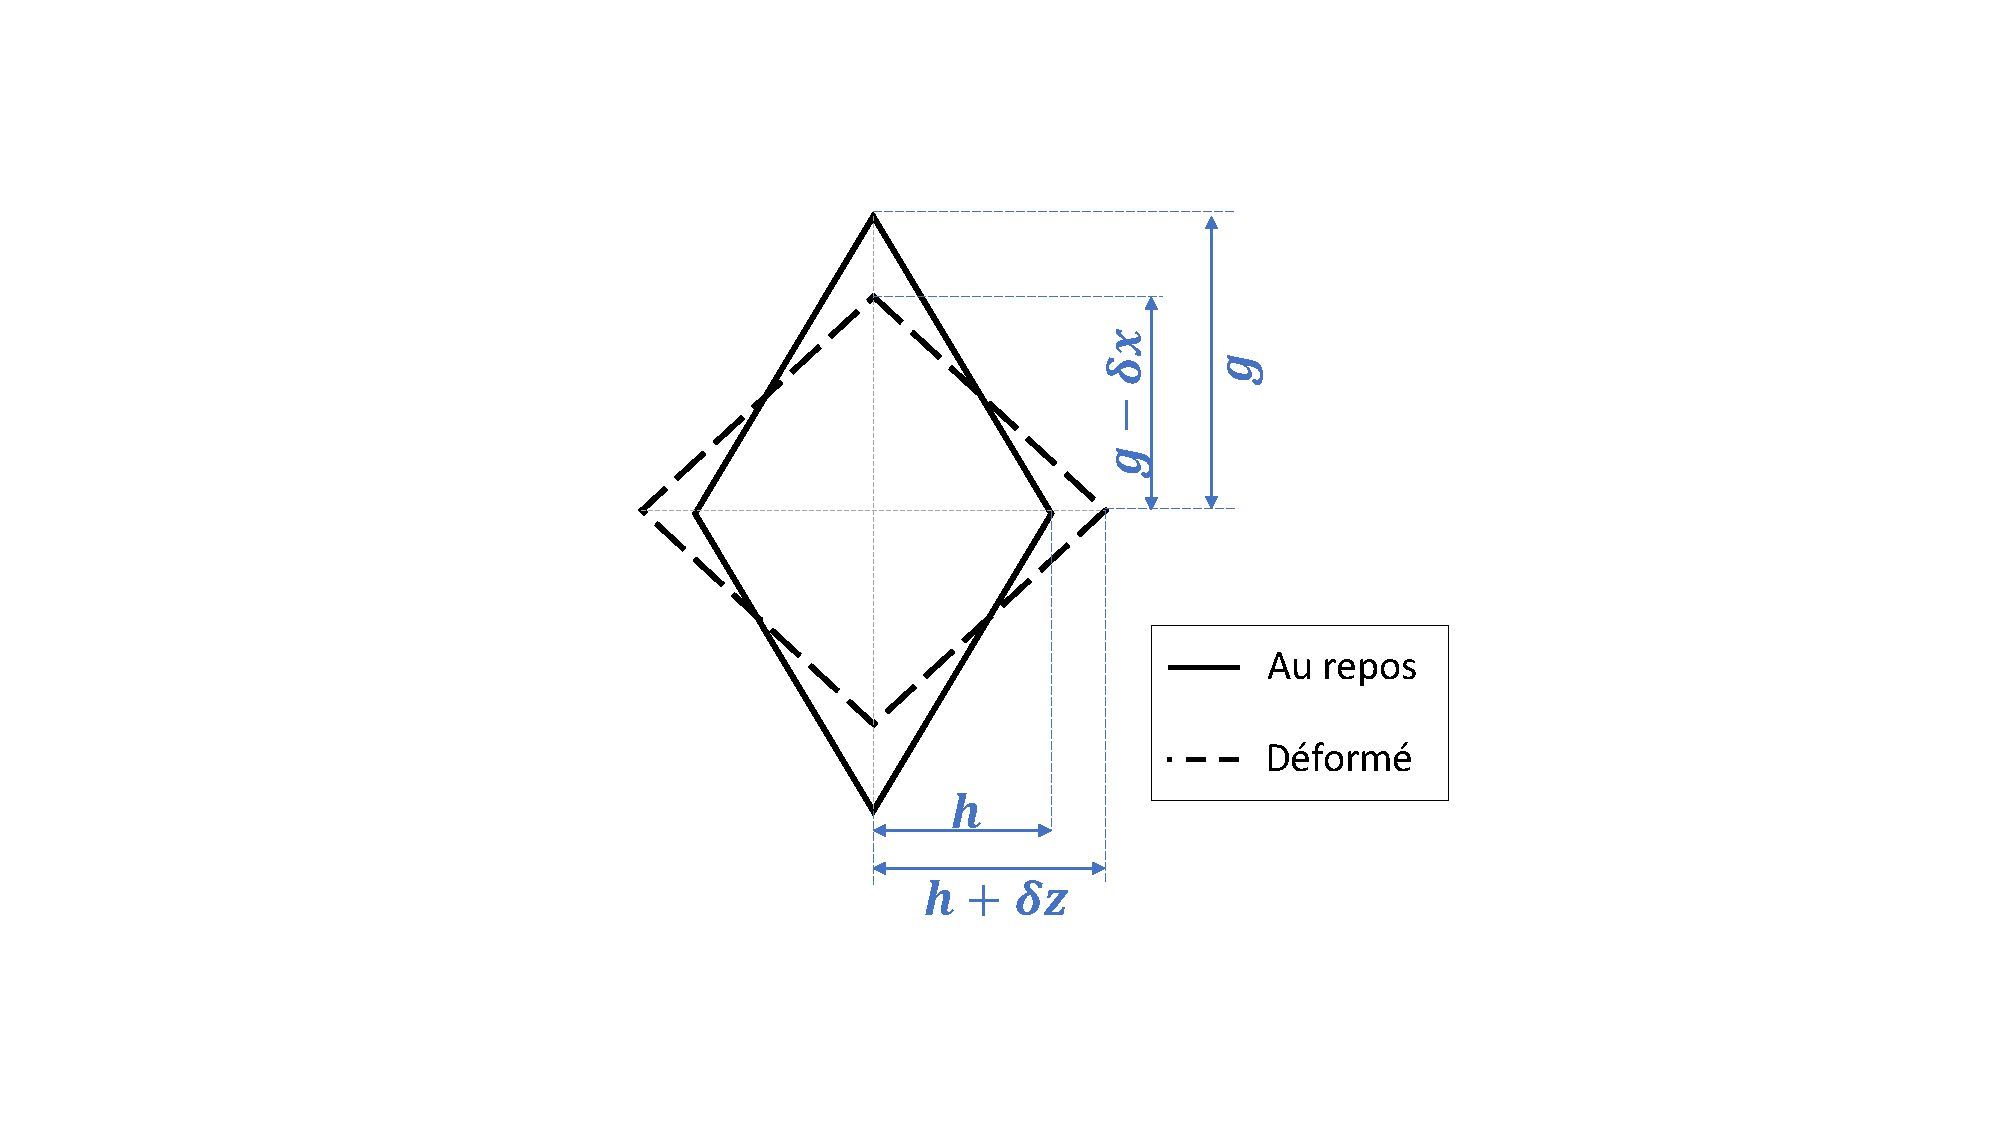
\includegraphics[trim={10.5cm 1cm 9cm 3cm},clip, 					                 width=\textwidth]{../Chap3/Figure/flextenseur_cinematique.pdf}
%	\caption{}
%	\label{fig:flextenseur_cinématique}
%	\end{subfigure}
%	\begin{subfigure}[b]{0.45\textwidth}
%    \captionsetup{justification=centering}
%	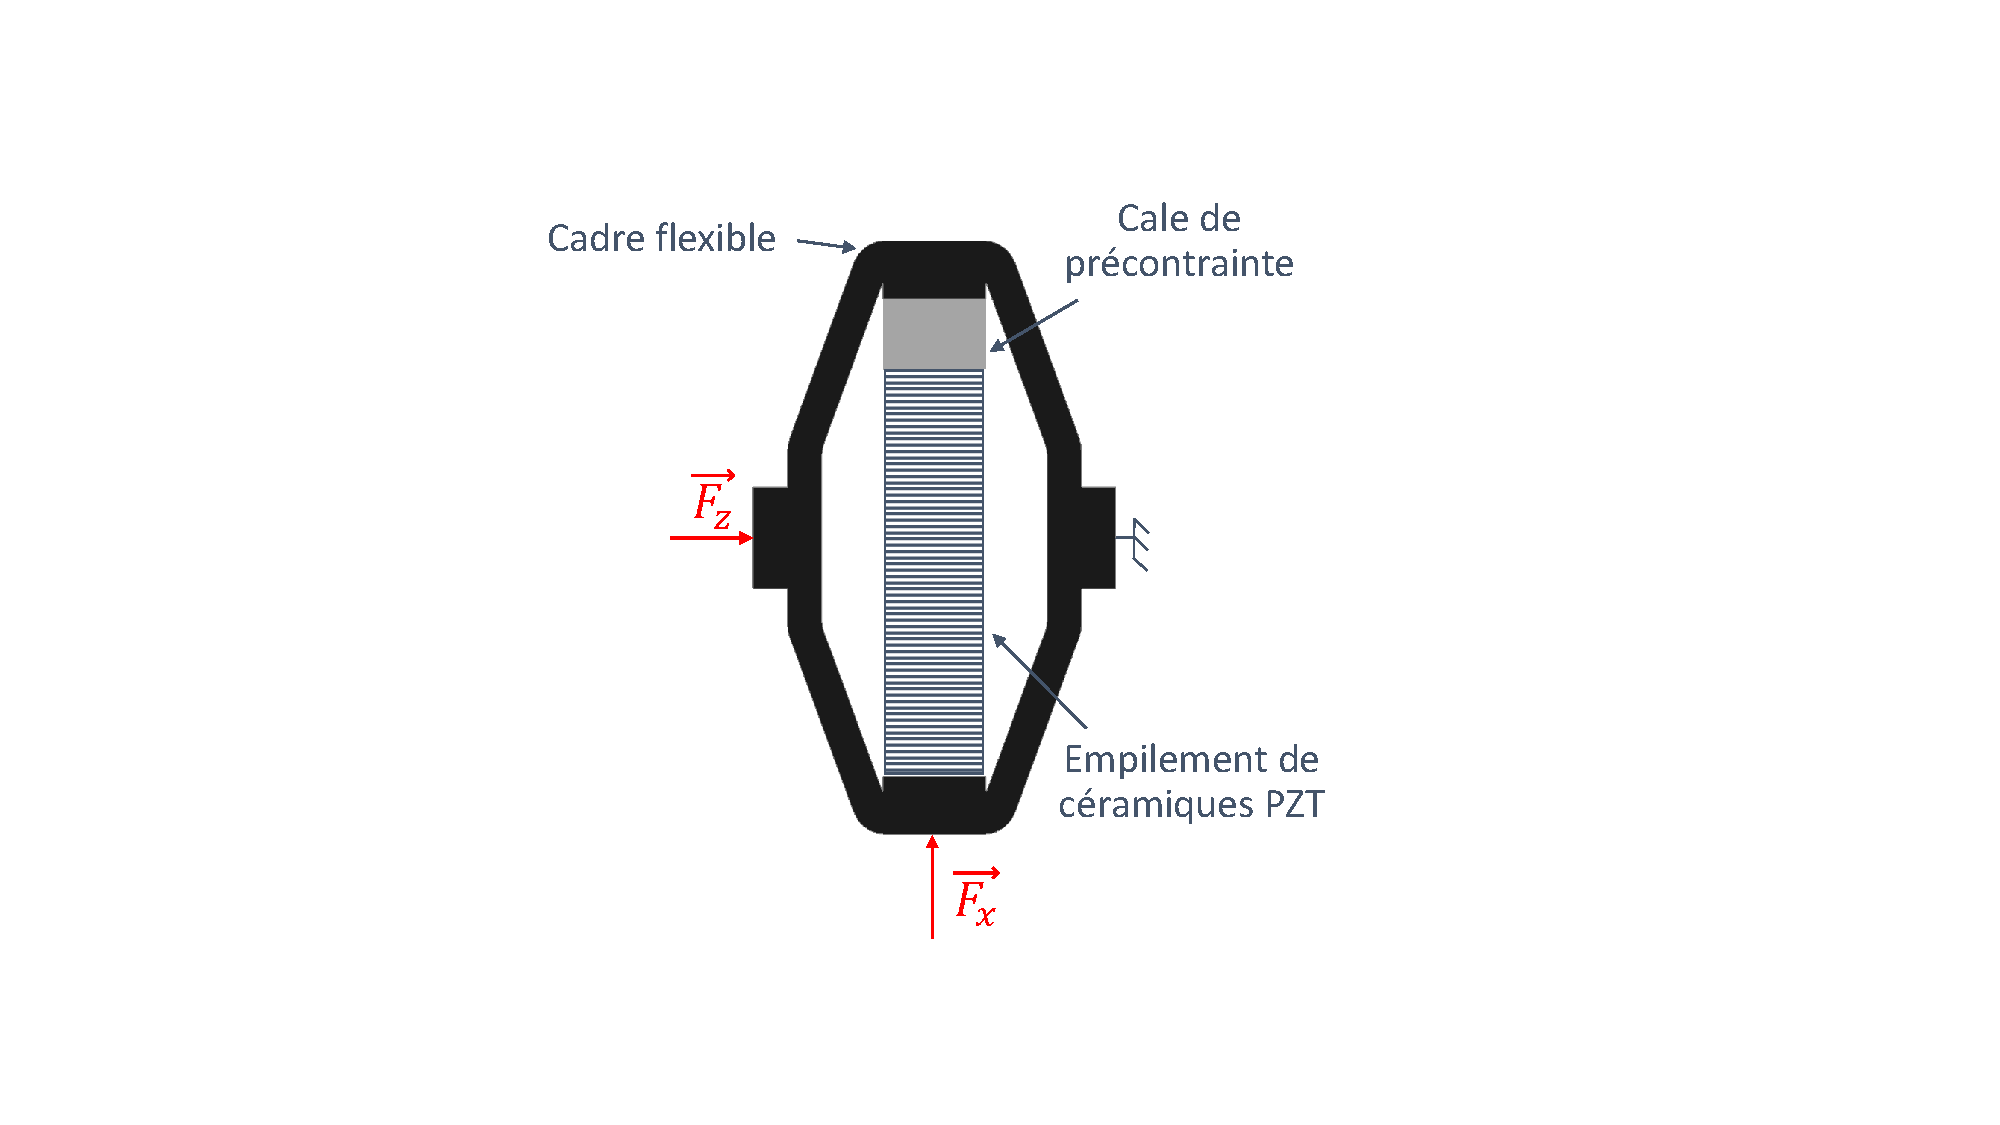
\includegraphics[trim={9cm 3cm 11.5cm 3cm},clip, 					                 width=\textwidth]{../Chap3/Figure/flextenseur_statique.pdf}
%	\label{fig:flextenseur_statique}
%	\caption{}
%	\end{subfigure}
%	\caption{(a) Comportement cinématique du flextenseur. (b) Comportement statique du flextenseur \cite{Zhou2013}}
%	\label{fig:flextenseur}
%\end{center}	
%\end{figure}
%%%%%%%%%%%%%%%%
%\begin{table}[!htbp]
%\centering
%%\rowcolors[]{2}{black!8}{}{
%\renewcommand{\arraystretch}{2}
%\begin{tabular}{c c}
%\rowcolor{blue!10}
%Titre1 & Titre2 \\
%\hline
%\hline
%élément 1 & élément 2\\ \hline
%\end{tabular}
%\end{table}
%%%%%%%%%%%%%%%%

\chapter{Conception et fabrication du convertisseur électromécanique : OB + GPA}
\label{ch:3_Conception et fabrication du convertisseur electromecanique : OB + GPA}
\minitoc
\newpage

%/!\/!\/!\/!\/!\/!\/!\/!\/!\/!\/!\/!\/!\/!\/!\/!\/!\/!\/!\/!\/!\/!\/!\/!\%
\section{Architecture générale}
\label{sec:3.1:Architecture generale}
%/!\/!\/!\/!\/!\/!\/!\/!\/!\/!\/!\/!\/!\/!\/!\/!\/!\/!\/!\/!\/!\/!\/!\/!\%
    %/////////////////////////////////////////////
	\subsection{Stratégie de conception de l'OB}
	\label{subsec:3.1.1:Strategie de conception de l'OB}
    %/////////////////////////////////////////////
\lettrine[lines=1]{L~'}{} e c\oe{}ur du dispositif de récupération d'énergie est constitué de l'OB intégrant le GPA. Il a donc été décidé de concevoir ces composants dans une logique de respect des critères d'encombrement. 

Afin de limiter les pertes mécaniques dans les liaisons de l'OB, nous avons introduit l'idée des liaisons pivots souples dans la structure, en remplacement des technologies dissipatives de type roulement. Une manière de réaliser ces liaisons est d'usiner l'OB directement dans un bloc monolithique pour se défaire des contraintes et problèmes éventuels liés à un assemblage. l'OB sera donc conçu dans l'optique d'être fabriqué à partir d'un bloc d'acier APX4 par électro-érosion. Cette méthode de fabrication nous permet d'avoir un contrôle précis sur les dimensions et par extension sur le comportement mécanique de l'oscillateur.

Les PHs et VH doivent s'intégrer autour de la masse dynamique de l'OB. Pour cela, il est préférable de prévoir un cadre rigide adapté à la mise en position relative et au maintien en position de ces composants, en accord avec les paramètres calculés lors du pré-dimensionnement (tab. \ref{tab:parametres électromécaniques} et \ref{tab:parametres_hydrauliques}).

Il sera par ailleurs utile d'assurer la possibilité de démontage du GPA, afin de permettre un éventuel remplacement si celui-ci est endommagé.		
    %/////////////////////////////////////////////
	\subsection{Architecture de l'OB}
	\label{subsec:3.1.2:Architecture de l'OB monobloc}	
    %/////////////////////////////////////////////
La figure \ref{fig:moboloc+GPA} présente la vue de face, ainsi que la vue isométrique du premier prototype fabriqué. Celui-ci a été conçu pour répondre aux besoins d'intégrabilité du GPA, des VH et du PH. La conception est pensée pour faciliter les caractérisations expérimentales. Pour cela, le mécanisme de réglage du niveau de flambement $x_0$ consiste en la mise en série d'un roulement et d'une vis micrométrique couplés par deux adaptateurs de diamètre représentés en bleu sur la figure \ref{fig:moboloc+GPA}.
\begin{figure}[!htbp]
\begin{center}
	\begin{subfigure}[b]{0.59\textwidth}
    \captionsetup{justification=centering}
	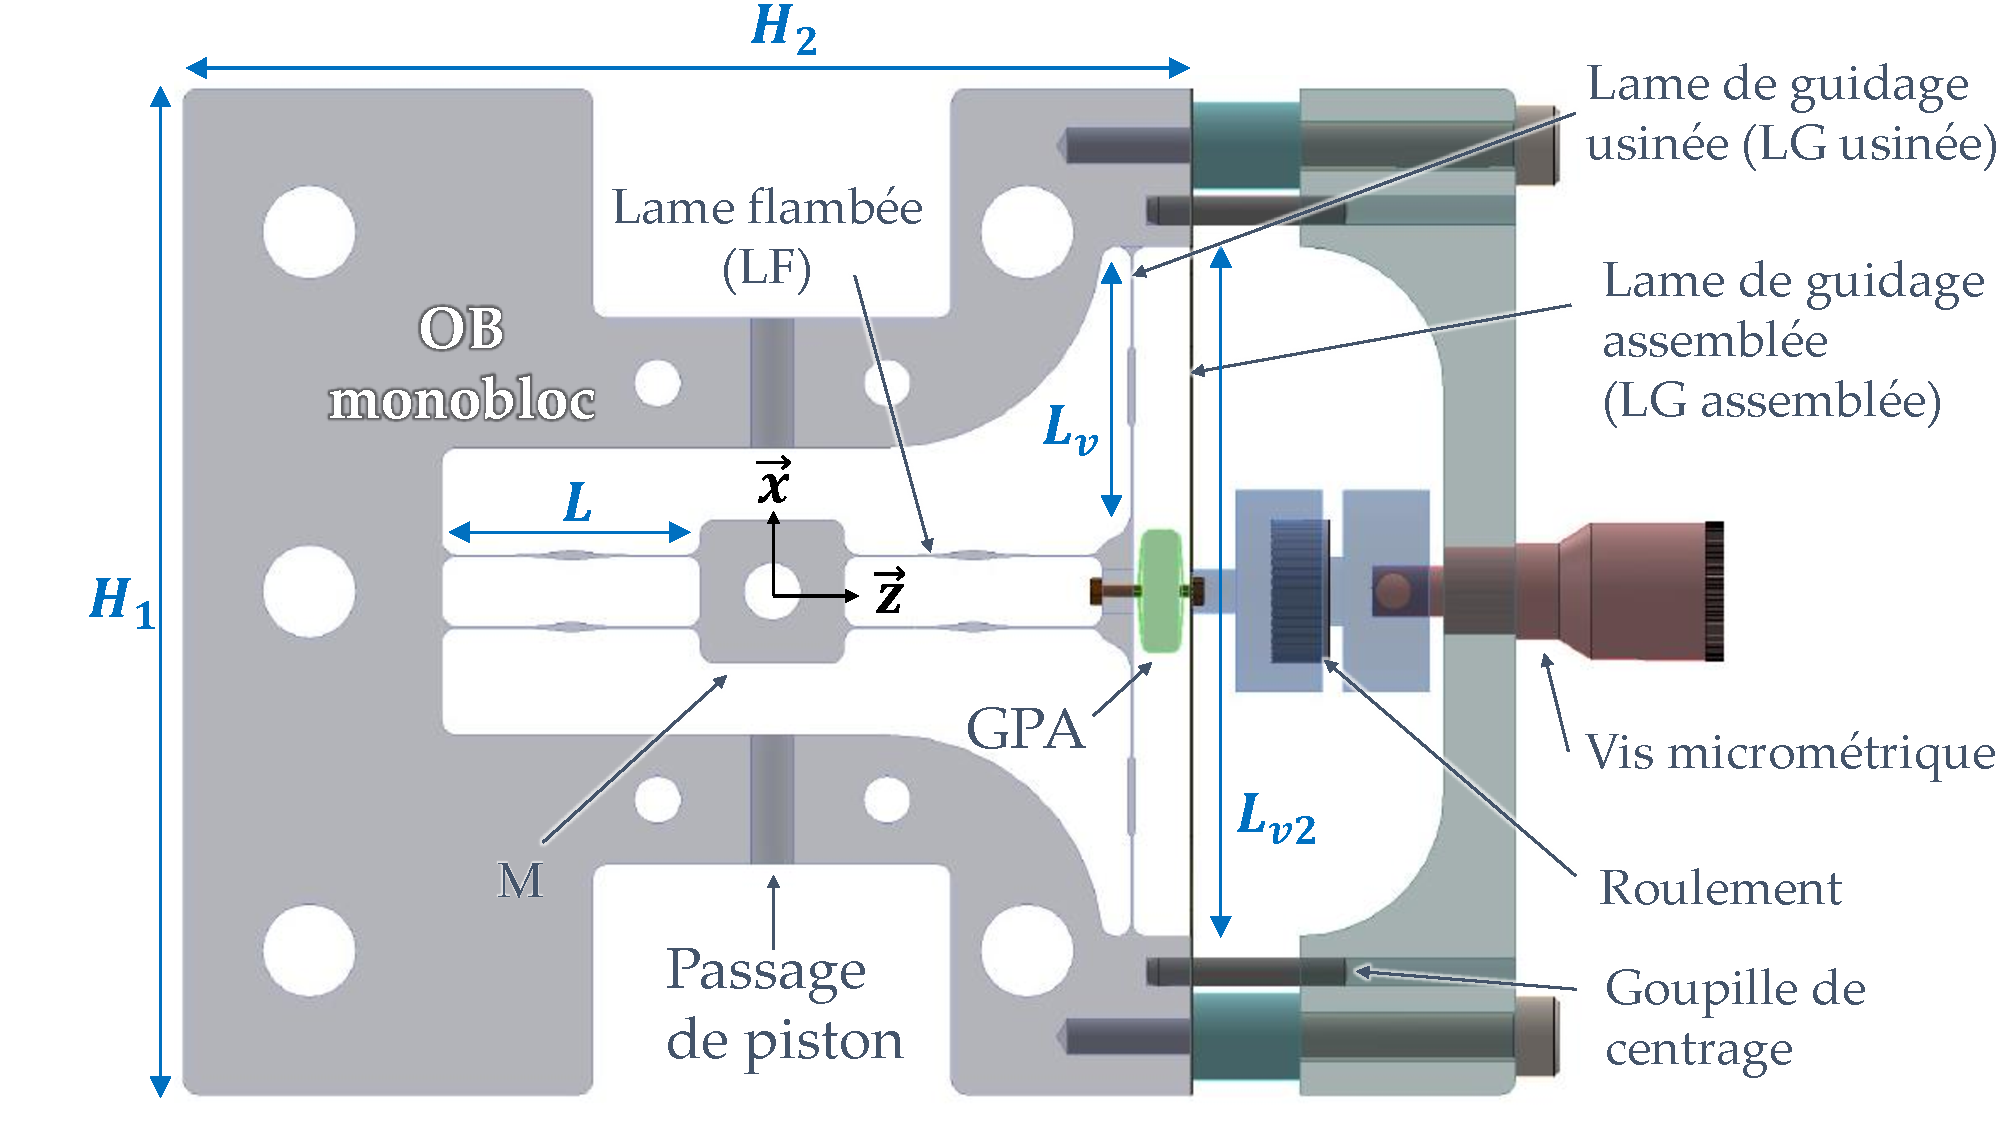
\includegraphics[trim={1.4cm 0cm 0cm 0cm},clip, width=\textwidth]{../Chap3/Figure/monobloc+GPA_face.pdf}
	\caption{Vue de face}
	\label{fig:moboloc+GPA_face}
	\end{subfigure}
	\begin{subfigure}[b]{0.4\textwidth}
    \captionsetup{justification=centering}
	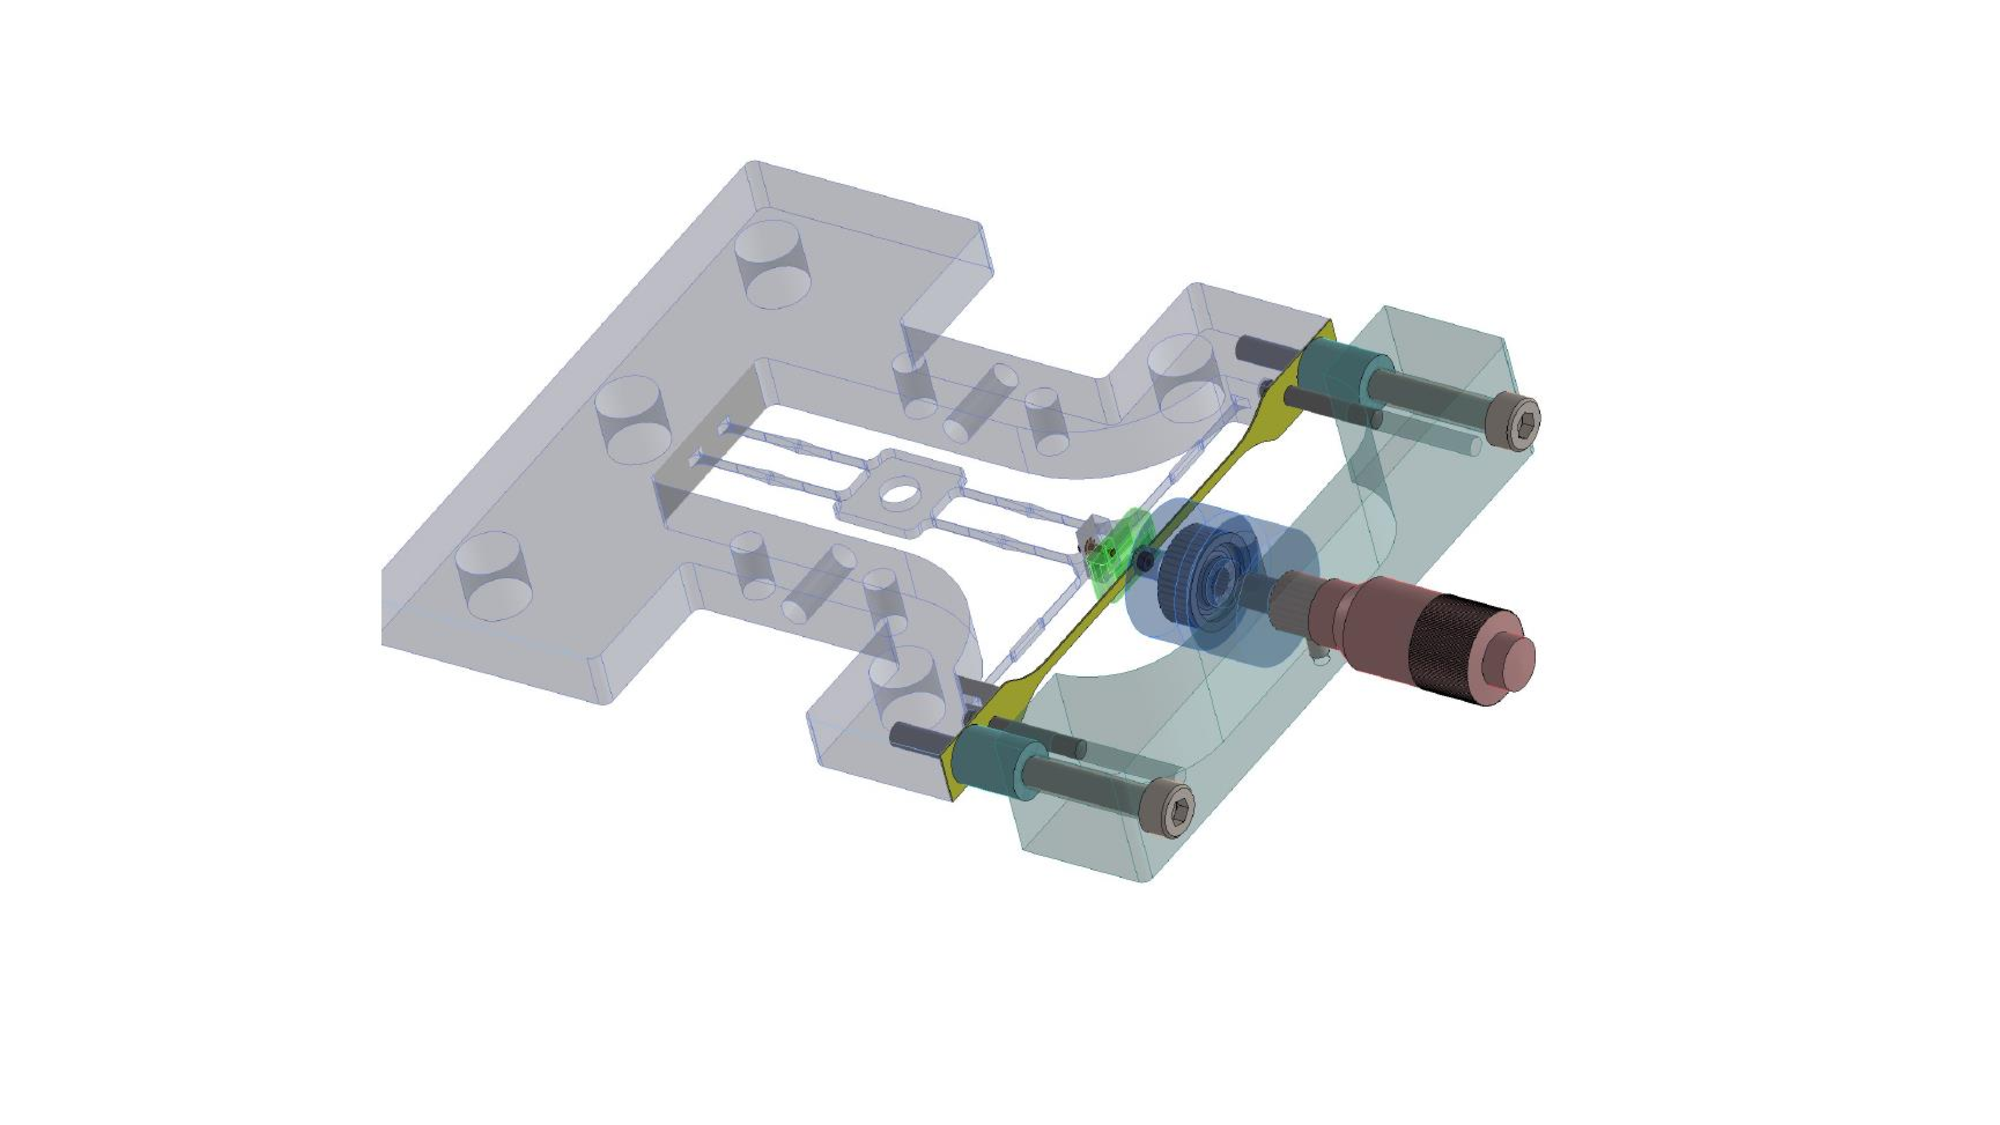
\includegraphics[trim={6cm 3cm 7.5cm 2.6cm},clip,width=\textwidth]{../Chap3/Figure/monobloc+GPA_iso.pdf}
	\label{fig:moboloc+GPA_iso}
	\caption{Vue isométrique}
	\end{subfigure}
	\caption{Architecture générale de l'OB intégrant le GPA et le réglage de flambement}
	\label{fig:moboloc+GPA}
\end{center}	
\end{figure}
%%%%%%%%%%%%%%%%

Le cadre extérieur est d'épaisseur 6mm afin d'être suffisamment rigide. Il sert de support pour accueillir les composants environnants (pistons notamment). La partie oscillante est d'épaisseur 1.2mm (ce paramètre est défini par la rigidité des 4 lames flambées (LFs), dont le dimensionnement est explicité dans la section qui suit). La masse centrale est percée pour pouvoir ajouter des lests supplémentaires, nous permettant ainsi de modifier la valeur de $m$. Deux perçages sont prévus dans l'alignement de M, afin d'accueillir les tiges des pistons hydrauliques. La dégagement près des passages de tiges servira à accueillir le corps de PHs, dont la documentation technique est donnée en annexe \ref{Ann:2_Vérin SMC série MQP}. Enfin, les deux lames de guidage (LGs) pourront empêcher toute rotation indésirable du GPA autour de l'axe $\vec{y}$.

La taille du bloc est de $H_1$ x $H_2$ = 70x70mm et la longueur d'une LF vaut $L=16$mm. Une mise en plan complète de l'OB monobloc est présentée dans l'annexe \ref{Ann:1_mise en plan OB}.
 
    %/////////////////////////////////////////////
	\subsection{Stratégie de conception des lames}
	\label{subsec:3.1.1:Stratégie des lames}
    %///////////////////////////////////////////// 
Afin de faire fabriquer un OB conforme aux caractéristiques mécaniques attendues, il est nécessaire de dimensionner les LGs et LFs. Les outils analytiques de la théorie des poutres, ainsi qu'un modèle EF simplifié de la structure de l'OB ont alors permis de calculer les dimensions géométriques de ces lames. Le tableau \ref{tab:parametres_lames} référence les résultats issus des calculs et simulations.    
%%%%%%%%%%%%%%%%%
\begin{table}[!htbp]
	\centering
	% \resizebox{\textwidth}{!}{%
	\rowcolors[]{2}{black!8}{}{
		\begin{tabular}{l|c|c}
			\rowcolor{blue!10}
			\toprule
			\textbf{Définition du paramètre} & \textbf{Symbole}    & \textbf{Valeur [Unité]} \\
			\midrule
			Module d'Young de l'acier APX4         & $E$                       & 211 [GPa]                     \\
			Résistance élastique de l'acier APX4   & $Re_{APX4}$               & 955 [MPa]                     \\
			Dimensions d'une LF                      & $L$ x $l$ x $e$           & 16x0.07x1.2 [mm]              \\
			Dimensions de la LG usinée             & $L_{v}$ x $l_{v}$ x $e$   & 17.5x0.07x1.2mm [mm]          \\
			Dimensions de la LG montée             & $L_{v2}$ x $l_{v2}$ x $e$ & 48x0.1x1.2mm [mm]             \\
			Raideur en rotation d'une liaison souple & $K_{\varphi}$             & 0.006 [Nm/rad]                   \\
			Raideur en flexion de la LG usinée     & $K_{LG}$                   & 190 [N/m]                     \\
			Raideur du GPA                         & $K$                       & 252 [kN/m]                    \\
			\bottomrule
		\end{tabular}}
	\caption{Définition et valeur des paramètres matériau, géométriques et mécaniques de l'OB monobloc}
	\label{tab:parametres_lames}
\end{table}
%%%%%%%%%%%%%%%%%%%%% 

Plusieurs aspects sont pris en compte pour la conception des différentes lames, dont une vue détaillée est proposée en annexe \ref{Ann:1_mise en plan OB}.

Le fonctionnement de l'OB induit la flexion des LGs et des LFs. Afin d'éviter les concentrations de contraintes aux points d'encastrement de ces dernières, des congés de 1mm de rayon ont été ajoutés. 

La faible largeur $l$ est issue du dimensionnement des LFs qui sera explicité dans la prochaine section. La longueur $L$ quant à elle découle du dimensionnement préliminaire de l'OB dans le respect des critères d'encombrement, ainsi que du niveau d'énergie disponible dans le gisement (0.79mJ d'après l'équation éq. \ref{eq:Energie_max_oreille}). Ces dimensions spécifiques ont pour conséquence l'addition d'épaississements au centre des lames usinées dans le bloc d'acier APX4. Ce choix de conception répond en effet à une problématique liée aux tolérances de fabrication. Le maintien de l'intégrité de la géométrie conçue avec les dimensions $l$ et $L$ calculées peut en effet être difficile lors de l'usinage de l'OB. Malgré le fait que l'usinage par électro-érosion offre de faibles tolérances dimensionnelles \cite{Rajurkar1997}, il est probable que les contraintes résiduelles au passage du fil de découpe induisent de légers flambements locaux sur les lames. Cela aurait pour conséquence de modifier le comportement mécanique de l'OB. Cela a notamment été observé dans les travaux de thèse de T. Huguet \cite{Huguet2019} sur des prototypes issus du même procédé de fabrication. Les épaississements des LFs et des LGs ont alors été dimensionnés en respectant leurs CdC respectifs, que nous présentons dans la suite de ce chapitre.
%/!\/!\/!\/!\/!\/!\/!\/!\/!\/!\/!\/!\/!\/!\/!\/!\/!\/!\/!\/!\/!\/!\/!\/!\%
	\section{Dimensionnement des lames flambées par approche EF}
	\label{sec:3.3:Dimensionnement des lames flambees par approche en EF}
%/!\/!\/!\/!\/!\/!\/!\/!\/!\/!\/!\/!\/!\/!\/!\/!\/!\/!\/!\/!\/!\/!\/!\/!\%
    %/////////////////////////////////////////////
	\subsection{Cahier des charges}
	\label{subsec:3.1.3:Cahier des charges lames flambees}	
    %///////////////////////////////////////////// 
La littérature nous a permis d'estimer les niveaux d'énergies disponibles dans la déformation mécanique du conduit auditif (tab. \ref{tab:Bouchard_deltaPmax}). Le choix a été fait de dimensionner le système de façon à induire un seuil de pression minimal dans l'oreille($p_c=1$kPa), afin de se placer dans les conditions les plus défavorables. Le gisement énergétique et le contexte applicatif ont motivé le choix du GPA (APA50XS : ann. \ref{Ann:6_Documentation technique sur l'APA50XS Cedrat Technologies}), fixant alors la raideur $K$. D'autre part, la longueur $L$ a été fixée en accord avec le contexte applicatif. Ces choix dimensionnent la géométrie des LFs qui doivent donc respecter les critères suivants :
\begin{itemize}[label=$\circ$]
	\item La précontrainte à appliquer par la vis micrométrique sur le GPA, afin de satisfaire le niveau de flambement $x_0$, doit être inférieure à la valeur nominale de $F_{adm}=18N$ admissible d'après le document constructeur de l'APA50XS qu'on trouve en annexe \ref{Ann:6_Documentation technique sur l'APA50XS Cedrat Technologies}.
	\item Les LFs doivent travailler dans leur domaine élastique sur toute la plage de variation de $x_m$ estimée d'après les résultats de pré-dimensionnement issus des simulations du chapitre précédent (fig. \ref{fig:simu_pos_debit_Cf_pression_1CYCLE})
\end{itemize}

Nous démontrerons alors, à travers une première étude statique par EF, que la flexion des LFs se produit dans leur domaine de comportement élastique, avec les dimensions respectives du tableau \ref{tab:parametres_lames}. De plus, cette étude permet d'estimer la rigidité en rotation $K_{\varphi}$ pour une liaison souple. Celle-ci sera implémentée dans le modèle système établi dans le chapitre précédent.
 
Une seconde étude de flambement, reprenant l'architecture du modèle EF précédent, montrera que la charge appliquée sur le GPA reste bien inférieure à $F_{adm}$.
 
    %/////////////////////////////////////////////
	\subsection{Raideur en rotation et domaine élastique} 
    %/////////////////////////////////////////////
    	%*************
		\subsubsection{Présentation du modèle EF} 
		%*************	
Une première approche consiste à simuler le comportement statique de la structure globale au travers d'un modèle éléments finis. La configuration de l'étude, ainsi que les conditions aux limites, sont représentées sur la figure \ref{fig:ANSYS_Conditions_Initiales}. L'étude est faite en grandes déformations avec les caractéristiques matériau du tableau \ref{tab:parametres_lames}.\\
%%%%%%%%%%%
\begin{figure}[!htbp]
\begin{center}
    \captionsetup{justification=centering}
	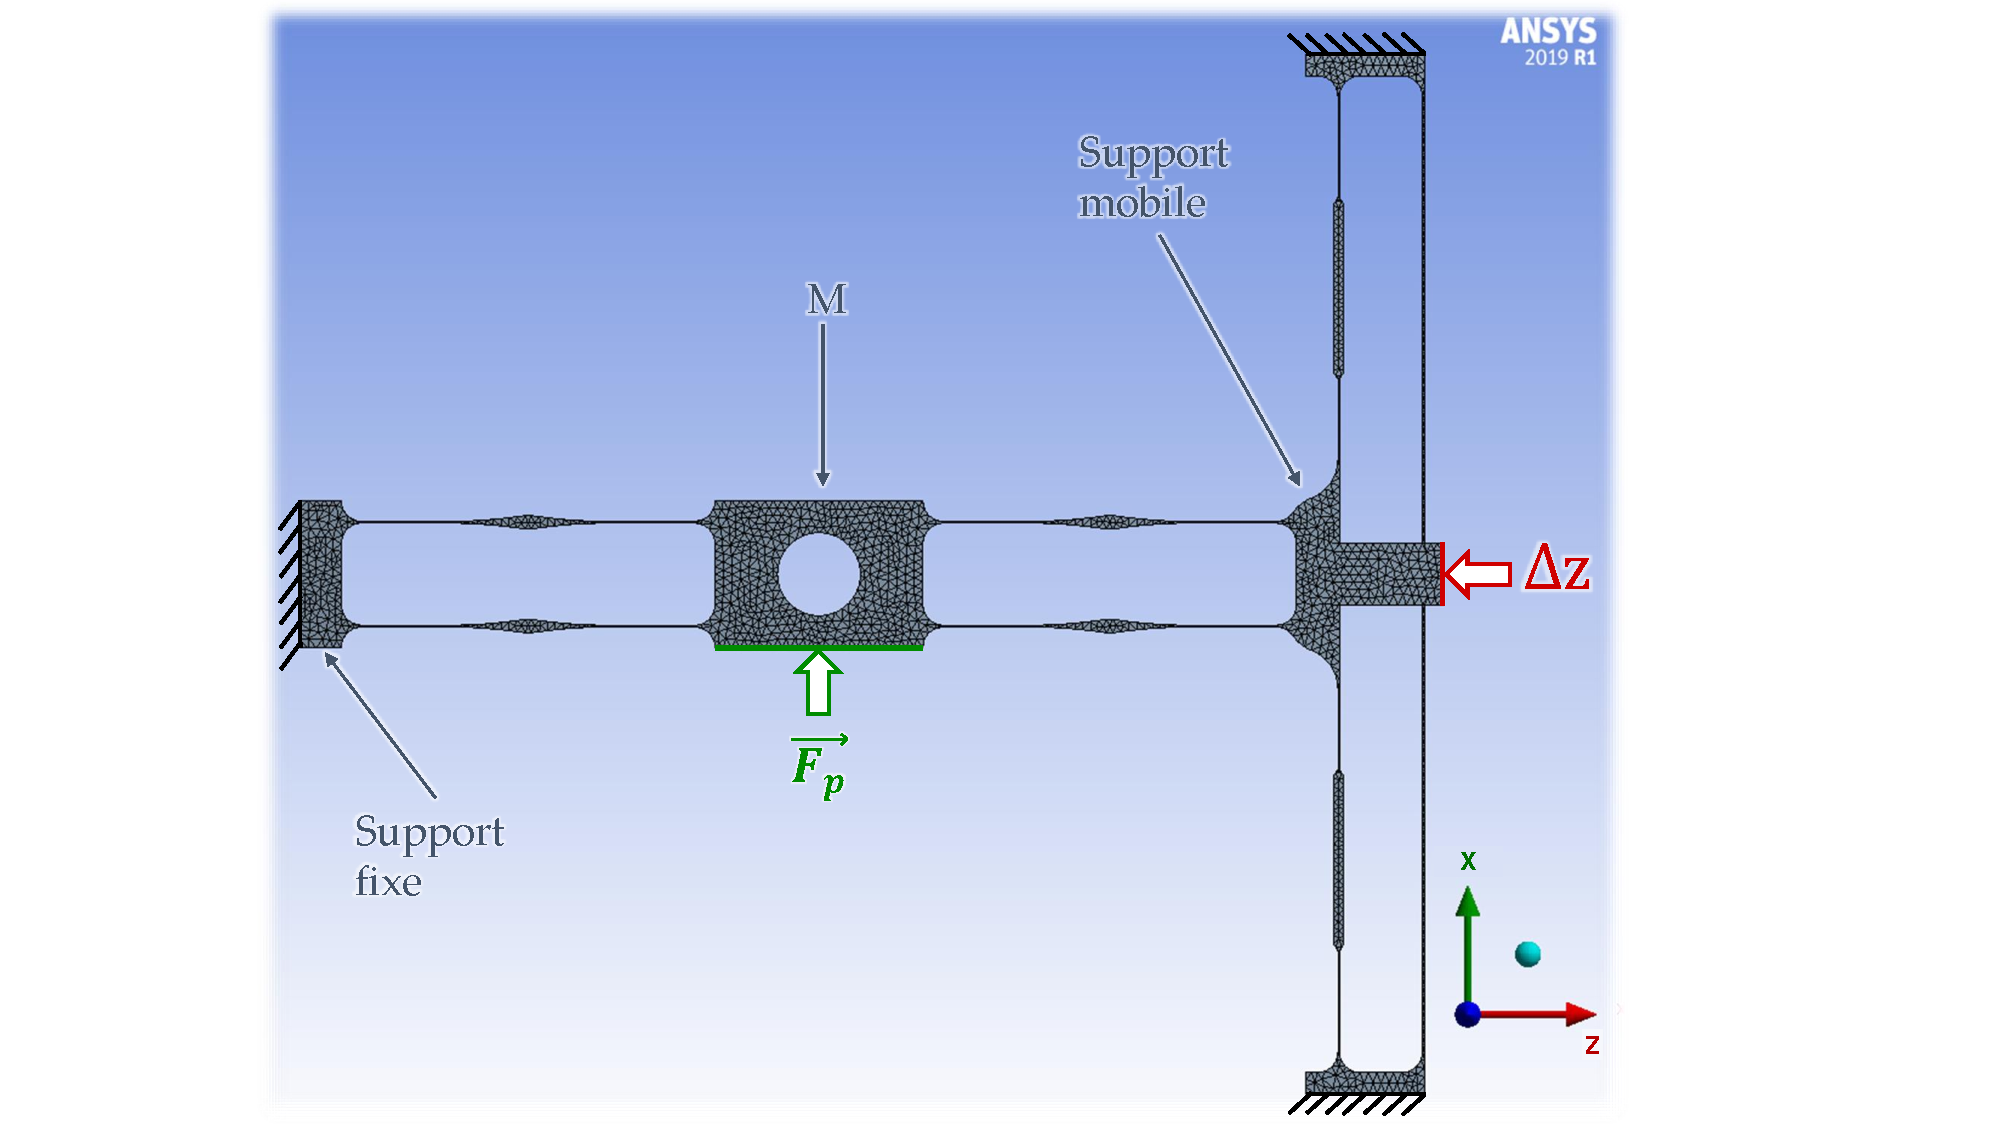
\includegraphics[trim={4.5cm 0cm 6.5cm 0cm},clip, width=0.8\textwidth]{../Chap3/Figure/ANSYS_Conditions_Initiales.pdf}
	\caption{Conditions aux limites de l'étude statique en EF de l'OB monobloc sur ANSYS}
	\label{fig:ANSYS_Conditions_Initiales}
\end{center}
\end{figure}
%%%%%%%%%%%
La géométrie a été simplifiée (suppression du cadre) pour faciliter le temps de calcul, tout en gardant les éléments essentiels au fonctionnement. La méthode de résolution se fait sur 100 incréments, dont les conditions initiales respectives sont égales aux conditions finales de l'incrément précédent. Le cadre extérieur de 6mm d'épaisseur est représenté par les trois supports fixes. Le GPA est modélisé par un bloc rigide nommé support mobile sur la figure \ref{fig:ANSYS_Conditions_Initiales}. Les efforts extérieures se résument en trois composantes principales :
\begin{itemize}[label=$\circ$]
\item Un déplacement nul aux supports fixes.
\item Un déplacement $\Delta z$ sur la surface se situant à l'extrémité droite du support mobile sur le plan $(xy)$. $\Delta z$ varie de 0 à -70µm suivant $\vec{z}$ sur 100 incréments linéaires.
\item La symétrie parfaite du système résultant d'une conception sans défauts géométriques rend impossible l'apparition du mode de flambement bistable qu'on recherche, si $\Delta z$ est la seule contrainte de déplacement. Une perturbation externe est donc nécessaire pour forcer le flambement vers l'une ou l'autre des positions stables haute et basse. De ce fait, on impose une force $\vec{F_p}$ appliquée sur la surface se situant en base de M sur le plan $(yz)$. $\vec{F_p}$ est constant égal à 3mN sur les 3 premiers incréments et vaut ensuite 0 sur les 97 incréments suivants. On s'assure par là que le flambement se produit du côté haut, dès les premiers incréments. Les suivants prennent chacun compte de la position stable de l'incrément précédent. La force $\vec{F_p}$ n'est donc plus nécessaire à partir du troisième incrément et la position finale n'est, par conséquent, pas affectée par celle-ci.
\end{itemize}

Lors des oscillations, la position de M varie de $\delta x$ autour de $x_0$. Il faut donc s'assurer que les lames se déformeront dans le domaine élastique sur cette plage de variation. Selon les simulations du chapitre précédent, on voit que la hauteur maximale d'oscillation de la masse est de $(x_m)_{max}=0.67$mm en imposant la position d'équilibre $x_0=0.49$mm. $(x_m)_{max}$ est atteint sur des déformations post-flambement du fait de l'inertie de M. Néanmoins, en première approximation, on suppose que la déformée des lames est comparable au cas d'une hauteur de flambement structurel initiale égale à $(x_m)_{max}$. La valeur de la précontrainte finale $\Delta z$ sera alors imposée de façon à flamber la structure à une hauteur supérieure à $0.67$mm.
    	%*************
		\subsubsection{Résultats des simulations EF} 
		%*************
Les figures \ref{fig:ANSYS_deplacement_X} et \ref{fig:ANSYS_Von_Mises} montrent respectivement le déplacement de la structure suivant l'axe $\vec{x}$ et la contrainte équivalente de Von Mises dans la position finale.

La figure \ref{fig:ANSYS_deplacement_X} montre que le déplacement de la masse en position finale est de $x_m=0.97$mm$\ >\ (x_m)_{max}$, comme souhaité. Connaissant la longueur des LFs ($L=16$mm), ainsi que la position de la masse à chaque incrément de déplacement, on peut extraire l'angle $\varphi$ d'après l'équation \ref{eq:Phi_calcul}.
\begin{equation}
\begin{split} 
\varphi\ =&\ \arctan {\biggl(\frac{x_m}{L}\biggr)} \\ 
\varphi\ \approx&\ \ \frac{x_m}{L}~~\text{car faibles déplacements} \\
\end{split}
\label{eq:Phi_calcul}
\end{equation}
%%%%%%%%%%%%%%%%%%%%%
\begin{figure}[!htbp]
\begin{center}
    \captionsetup{justification=centering}
	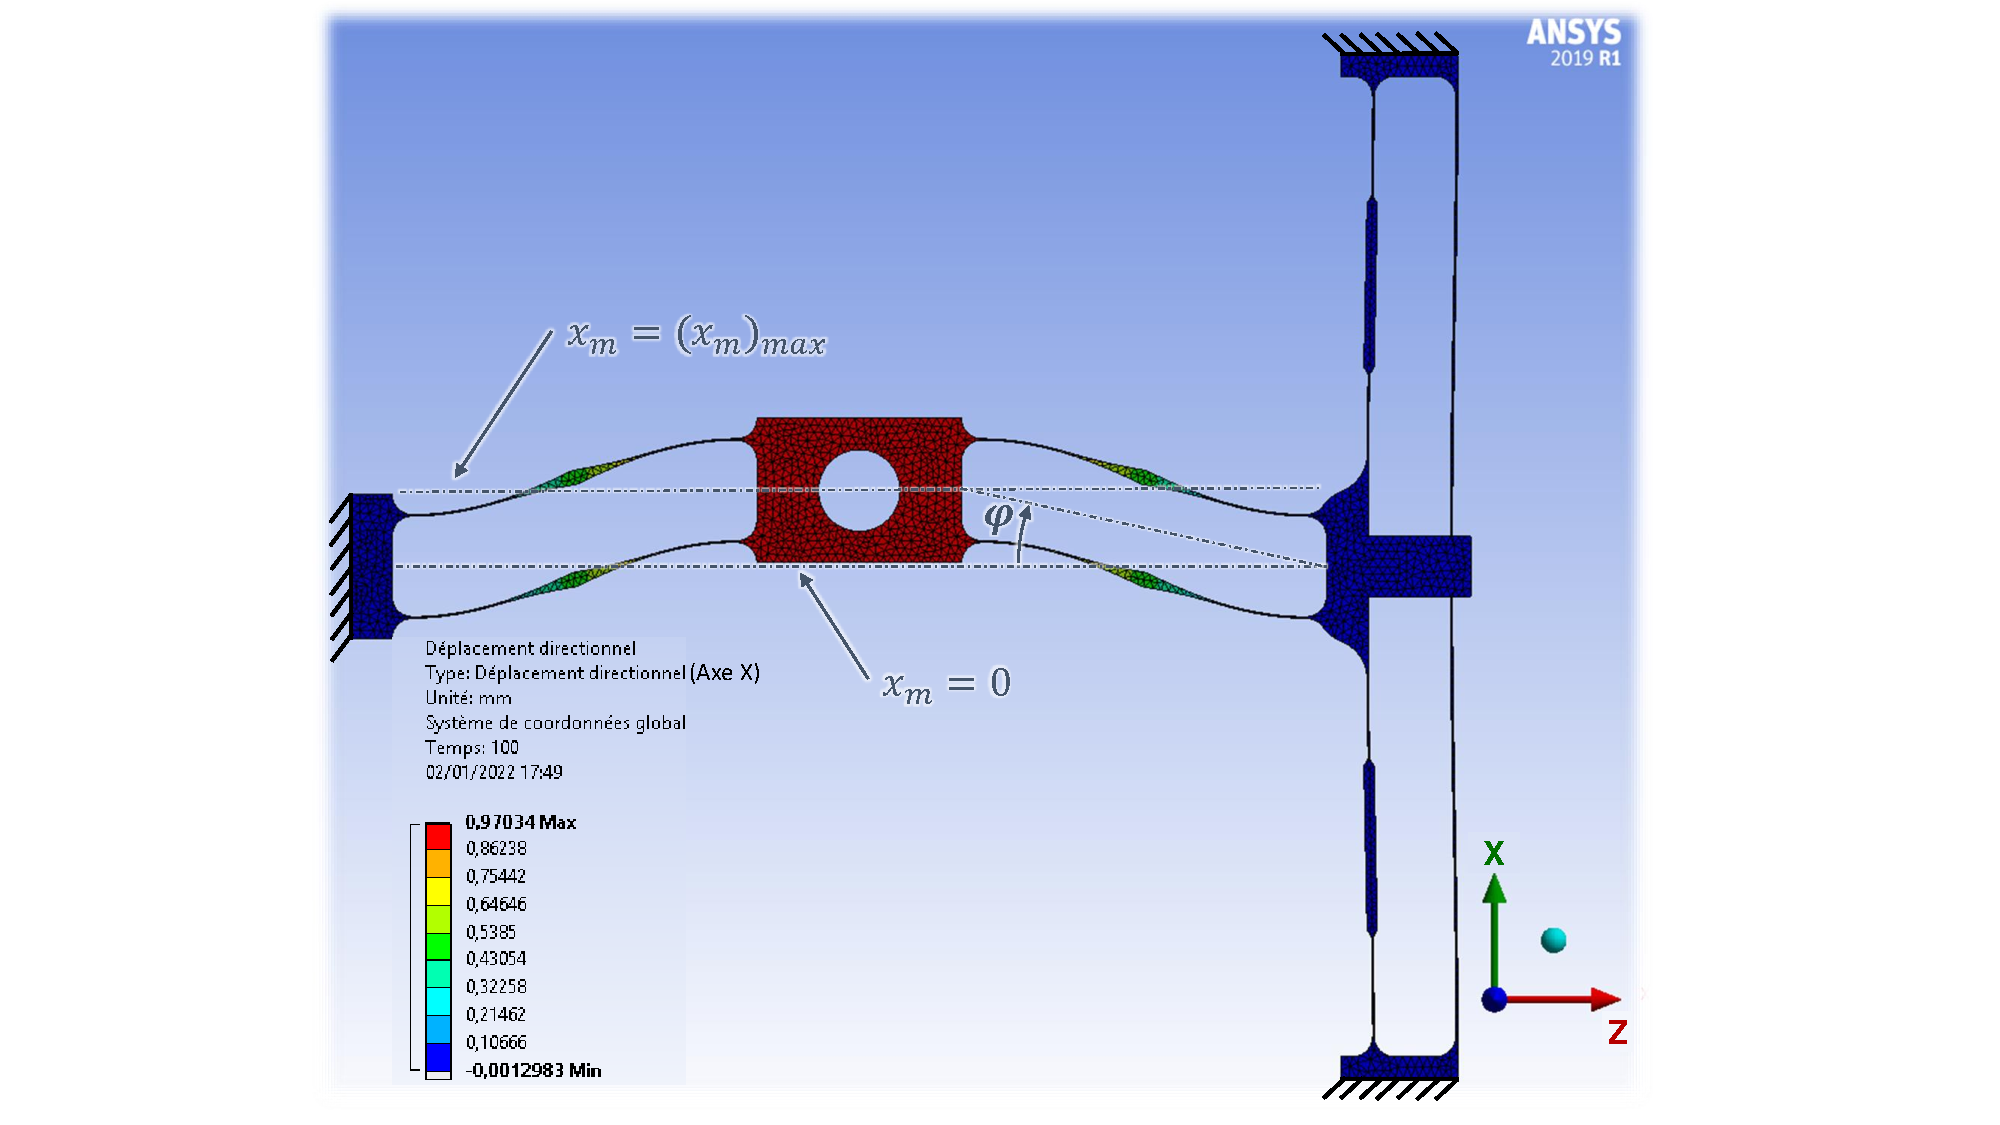
\includegraphics[trim={5.5cm 0cm 6cm 0cm},clip, width=0.8\textwidth]{../Chap3/Figure/ANSYS_deplacement_X.pdf}
	\caption{Déplacement de la structure monobloc suivant l'axe $\vec{x}$}
	\label{fig:ANSYS_deplacement_X}
\end{center}
\end{figure}
%%%%%%%%%%%

La contrainte maximale relevée sur les LFs est de ${\sigma}_{max} = 153$MPa comme on peut le voir sur la figure \ref{fig:ANSYS_Von_Mises}. On s'assure par là que la déformation a bien lieu dans le domaine élastique du matériau. La localisation exacte des centres instantanés de rotation n'est pas possible car les déformations sont réparties le long des portions fines des LFs. On peut néanmoins approximer leurs positions à l'extrémité des congés se situant aux points d'encastrement des lames. Cela induit une faible incertitude sur la valeur exacte de $L$ et pourra alors expliquer un écart entre les paramètres expérimentaux et théoriques.
 
L'énergie de déformation contenue dans la structure est majoritairement issue de la flexion aux liaisons souples, au vu de la répartition des contraintes (fig. \ref{fig:ANSYS_Von_Mises}). Sachant qu'on est capable d'extraire cette énergie pour chaque incrément de déplacement, on peut connaître son évolution selon la variation de $\varphi$. De plus, en cherchant la dérivée locale de l'évolution énergétique par rapport à l'angle $\varphi$, on peut remonter au moment de rappel que les lames exercent pour ramener la masse vers la position $x_m=0$ (eq. \ref{eq:définition_M_st}).
%%%%%%%%%%%
\begin{figure}[!htbp]
\begin{center}
    \captionsetup{justification=centering}
	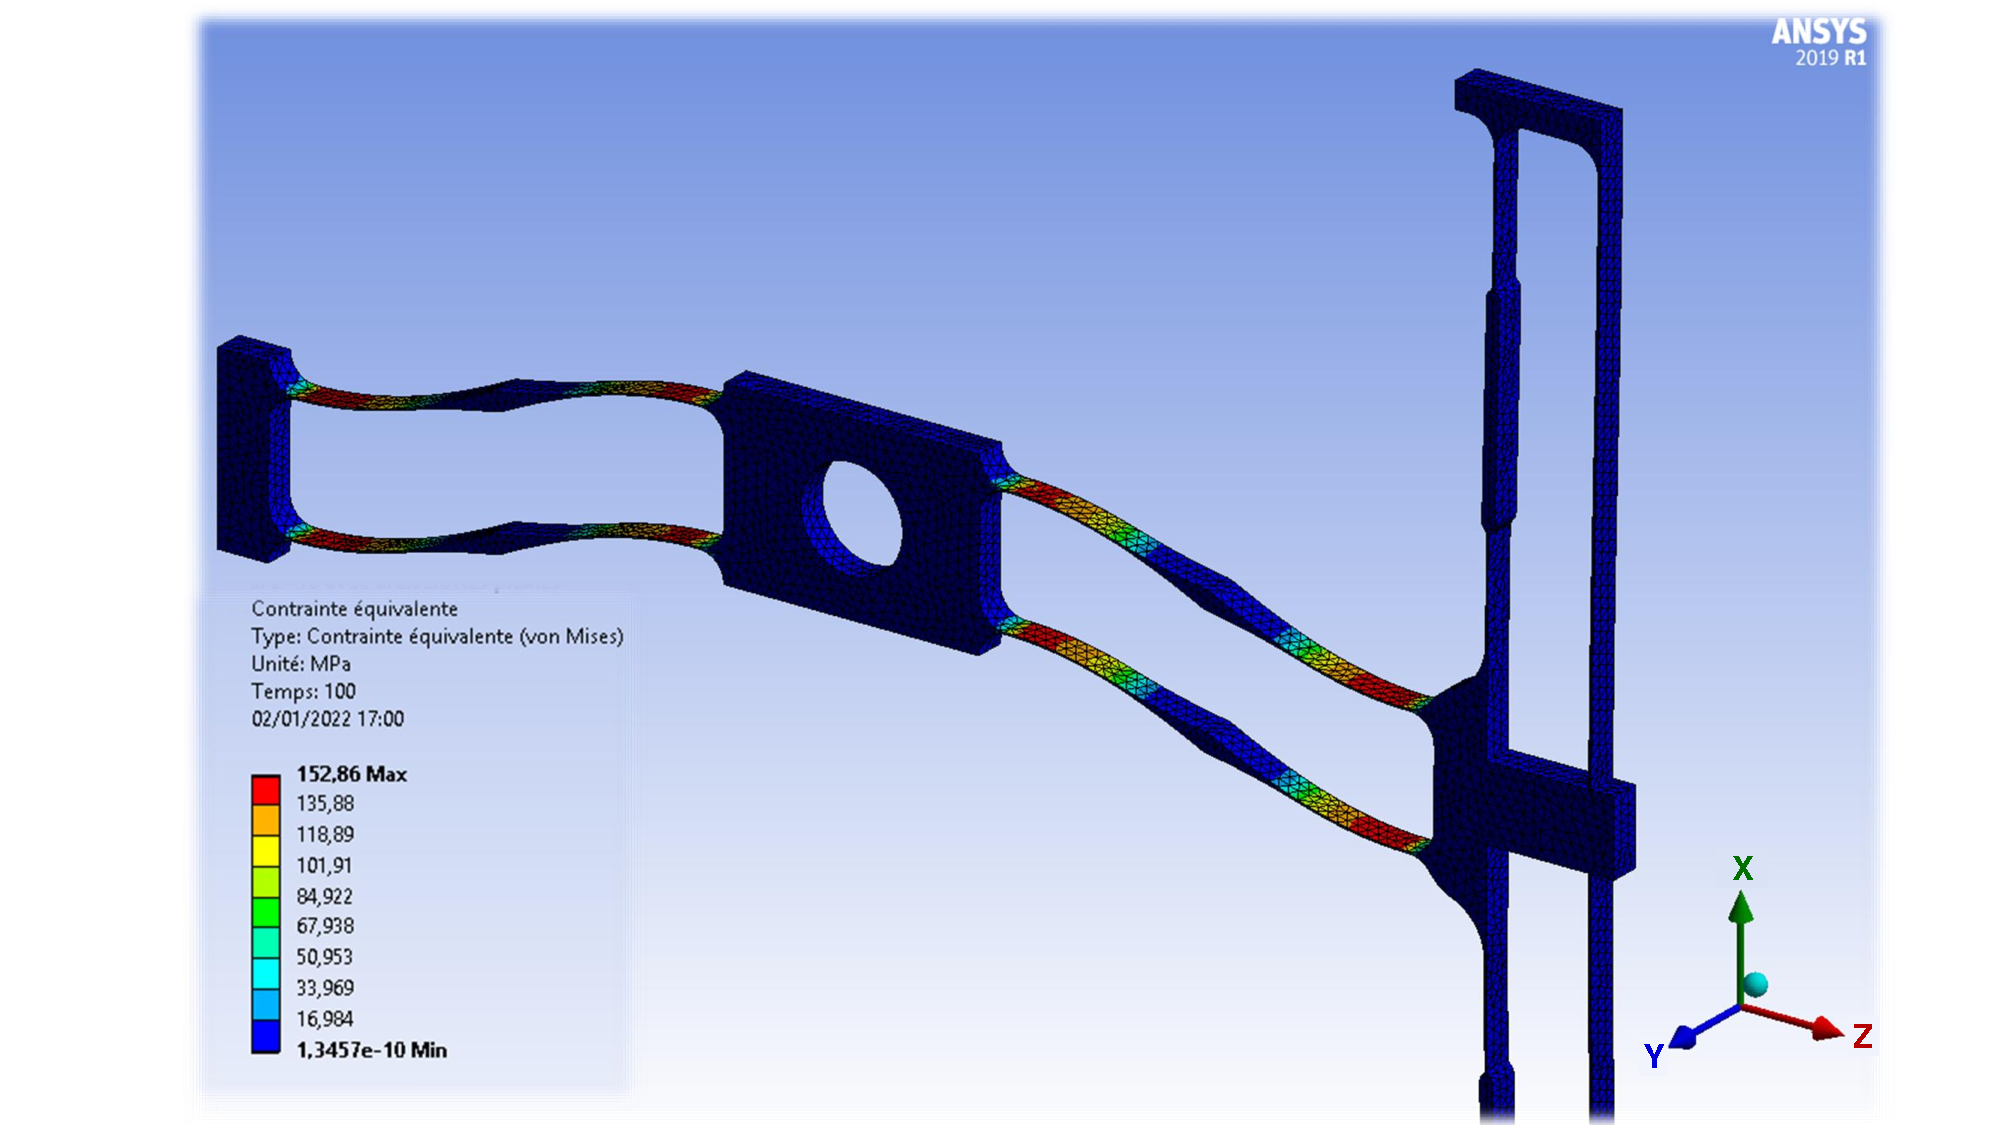
\includegraphics[trim={3.2cm 0cm 2cm 0cm},clip, width=0.8\textwidth]{../Chap3/Figure/ANSYS_Von_Mises.pdf}
	\caption{Contrainte équivalente de Von Mises dans la structure monobloc}
	\label{fig:ANSYS_Von_Mises}
\end{center}
\end{figure}
%%%%%%%%%%%
\begin{equation}
	M_{st} = \frac{d E_{st}}{d \varphi}
	\label{eq:définition_M_st}
\end{equation}
L'évolution de $M_{st}$ et $E_{st}$ est montrée sur la figure \ref{fig:ANSYS_energie+moment} en fonction de $\varphi$. Le comportement linéaire des liaisons pivot souples est clairement visible sur l'évolution de $M_{st}$. On peut alors extraire la rigidité $K_{st}$ en flexion pour toute la structure déformée avec l'équation \ref{eq:définition_K_st}.
\begin{equation}
		K_{st} = \frac{M_{st}}{\varphi}
		\label{eq:définition_K_st}
\end{equation} 
On s'assure bien de calculer le moment de flexion et la rigidité sur les données où la perturbation $\vec{F_p}$ est nulle et on obtient alors $K_{st} = 24$Nmm/rad, constant suivant $\varphi$ dans la plage de fonctionnement souhaitée. Dans le modèle établi au chapitre précédent, on considère 4 liaisons pivot (fig. \ref{fig:schema_cinematique1}). Une seule liaison pivot a une rigidité $K_{\varphi}$ qui peut alors s'exprimer à partir du résultat précédent avec l'équation \ref{eq:définition_K_phi}.
\begin{equation}
		K_{\varphi} = \frac{K_{st}}{4} = 6\ \text{Nmm/rad}
		\label{eq:définition_K_phi}
\end{equation}
%%%%%%%%%%%
\begin{figure}[!ht]
	\begin{center}
		\captionsetup{justification=centering}
		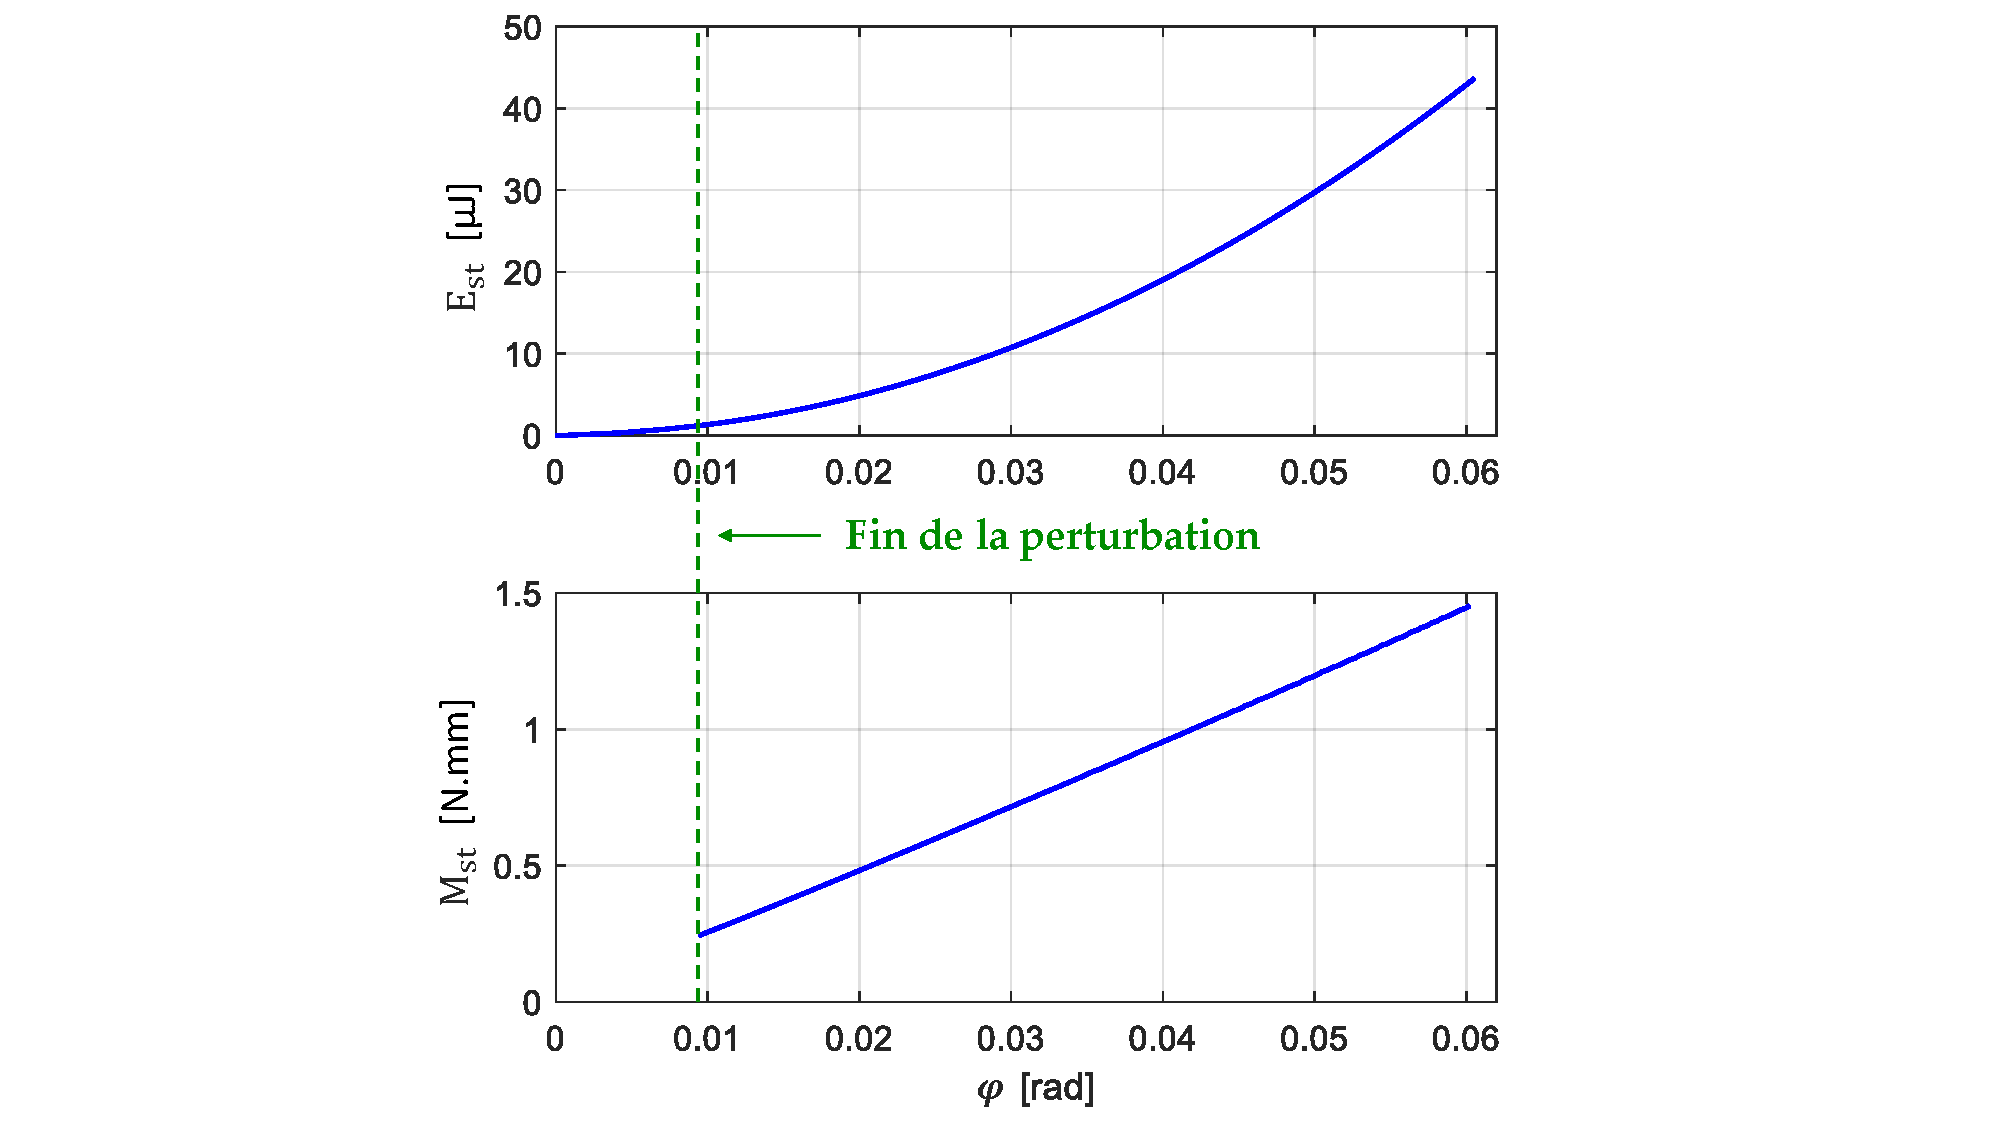
\includegraphics[trim={7cm 0cm 8cm 0cm},clip, width=0.7\textwidth]{../Chap3/Figure/ANSYS_energie+moment.pdf}
		\caption{Énergie de déformation de la structure et moment de rappel des liaisons pivot souples en fonction de l'angle de flexion $\varphi$}
		\label{fig:ANSYS_energie+moment}
	\end{center}
\end{figure}
%%%%%%%%%%%

Par ailleurs, l'annexe \ref{Ann:5_Dimensionnement analytique des lames de l'OB} propose une approche analytique pour le dimensionnement statique des LFs. Celle-ci est corrélée avec les résultats du modèle EF présentés dans cette section et les résultats sont quasiment similaires. 
	%///////////////////////////////////////////// 		
	\subsection{Précontrainte de flambement et limite structurelle}
	\label{sec:3.3.1_Limite structurelle et précontrainte de flambement}
    %/////////////////////////////////////////////		
Cette étude a pour but d'identifier la précontrainte nécessaire à appliquer à la structure afin de la flamber dans un configuration bistable similaire à celle illustrée sur la figure \ref{fig:ANSYS_Von_Mises}. La précontrainte pour l'induire devra correspondre à une force inférieure à la force $F_{adm}=18N$ admissible par le GPA. De plus, l'étude permettra d'estimer, au passage de M par la position $x_m=0$, l'effort limite de compression pouvant être supporté par les LFs, au delà duquel elles se déformeraient en flambage. Dans ce cas défavorable, au lieu de transmettre les efforts de compression, les LFs se plieraient aux points de rotation souples et absorberaient alors l'énergie qui aurait dû être emmagasinée dans le ressort du GPA.

Le modèle développé dans le chapitre précédent suppose que les LFs assurent le rôle des liaisons pivot élastiques. Nous avons validé cet aspect par l'étude statique. Le modèle analytique suppose aussi qu'entre les liaisons souples les lames sont infiniment rigides, assurant ainsi la meilleure transmission des efforts au GPA et maximisant de ce fait le coefficient de couplage du système. Nous allons vérifier que cette hypothèse est vraie avec les valeurs des paramètres du tableau \ref{tab:parametres_lames}.

La figure \ref{fig:schema_compression_GPA_ch4} illustre l'OB en position d'équilibre stable à $x_m=x_0$ et en position instable lorsque $x_m=0$. L'effort $F_{z,x_0}$ représente la précontrainte du GPA induisant le flambement en $x_0$ et $F_{z,0}$ représente la contrainte de compression subie par les LFs lorsque M passe par sa position instable.
%%%%%%%%%%%%%%%%%%%%%%%%%%%%%%%%%%%%	
\begin{figure}[!htb]
	\begin{center}
		\captionsetup{justification=centering}
		\includegraphics[trim={0cm 0cm 0cm 5cm},clip,width=0.8\textwidth]{../Chap3/Figure/schéma_compression_GPA_flambement.pdf}
		\caption{Détail d'une lame horizontale du prototype d'OB conçu}
		\label{fig:schema_compression_GPA_ch4}
	\end{center}
\end{figure}  
%%%%%%%%%%%%%%%%%%%%%%%%%%%%%%%%%%%%
$F_{z,0}$ est, par contre-réaction, la force élastique générée lors de la compression du GPA. Elle peut être évaluée en fonction de $x_0$ à travers l'équation \ref{eq:F_z ch4}. La figure \ref{fig:Fz(x0)} montre alors l'évolution de $F_{z,0}$ en fonction de $x_0$, pour $K$ et $L$ fixés (tab. \ref{tab:parametres électromécaniques}).
\begin{equation}
	F_{z,0}\ =\ K\ \Delta z\ =\  2K(\sqrt{({x_0}^2+L^2)}-L)
	\label{eq:F_z ch4}
\end{equation}
%%%%%%%%%%%%%%%%%%%%%%%%%%%%%%%%%%%%	
\begin{figure}[!htb]
\begin{center}
    \captionsetup{justification=centering}
	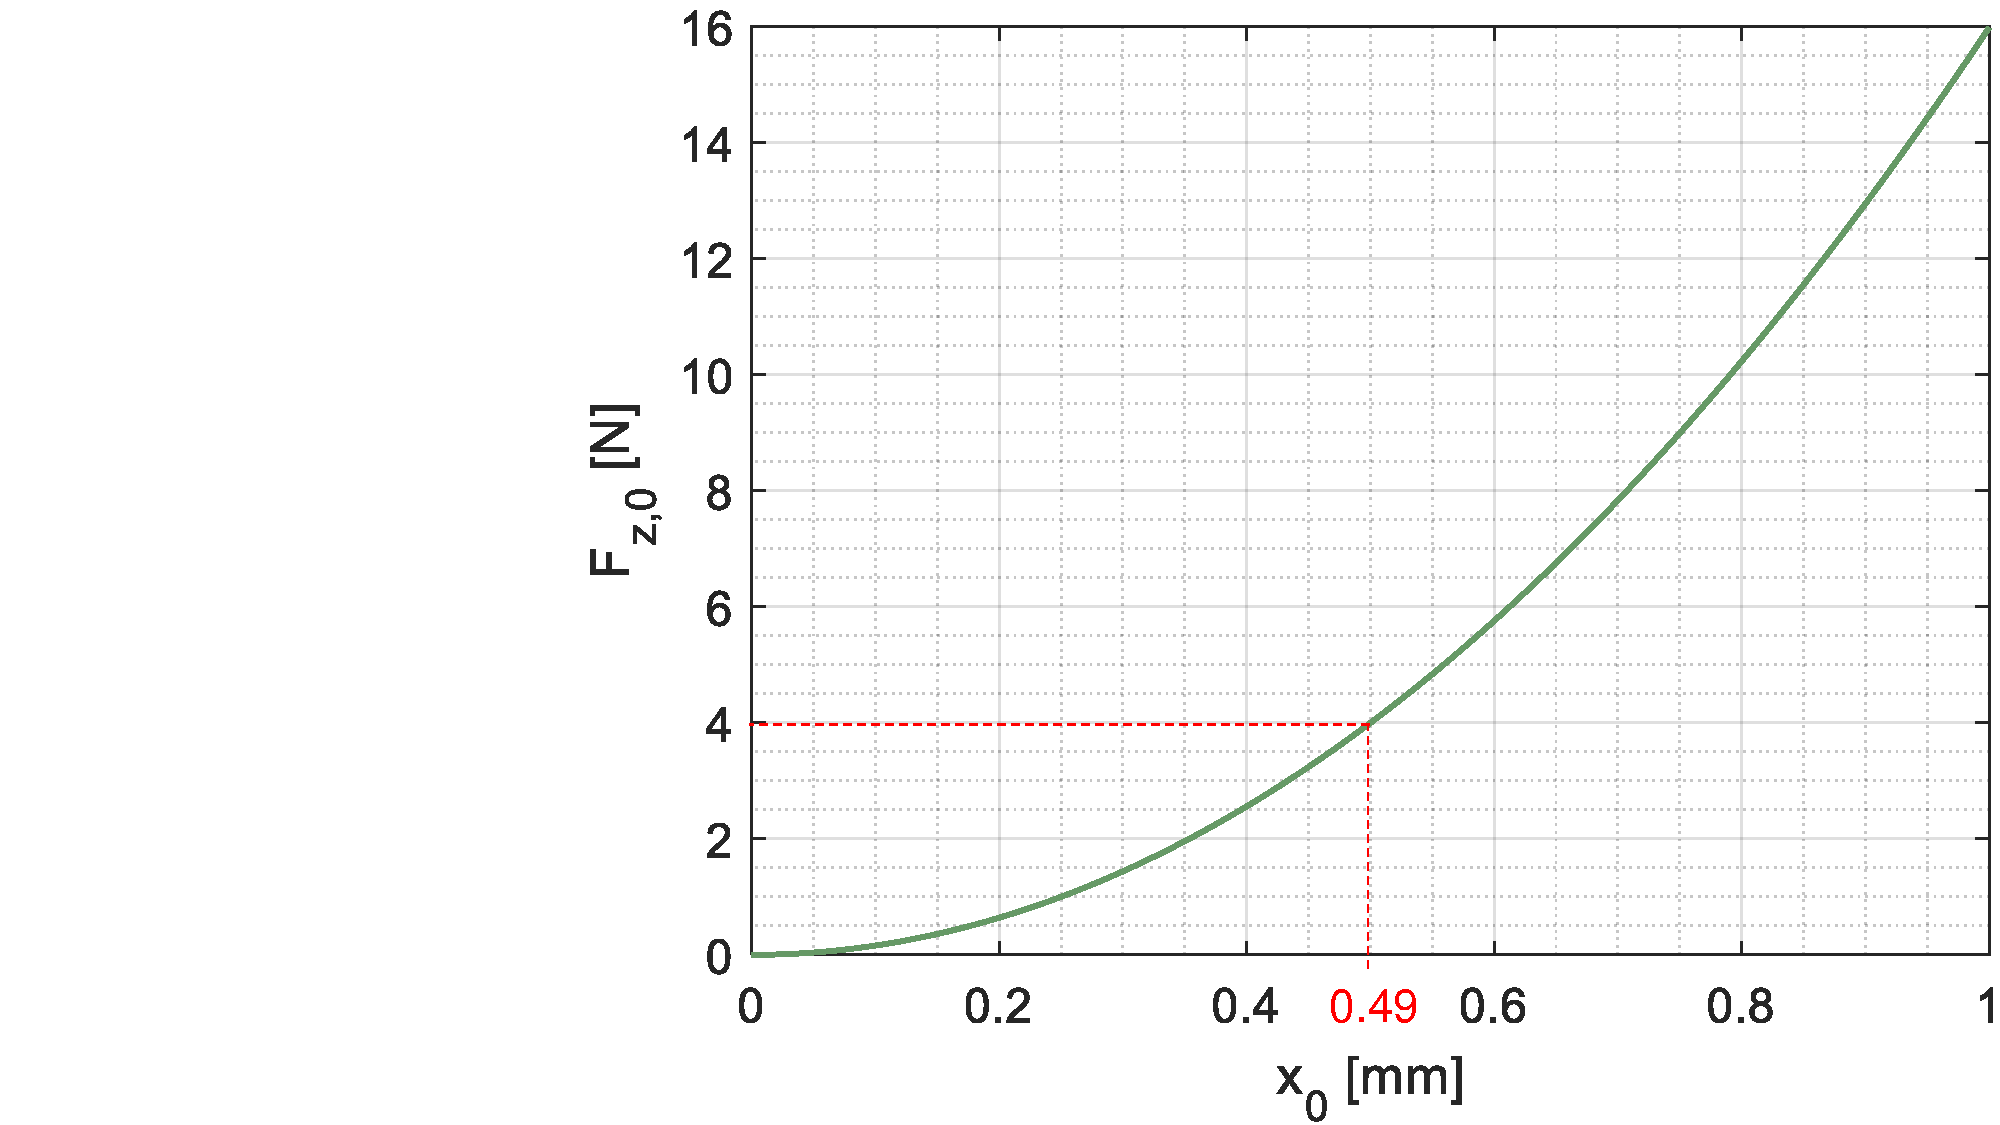
\includegraphics[trim={10cm 0cm 0cm 0cm},clip, 					                 width=0.5\textwidth]{../Chap3/Figure/Fz(x0).pdf}
	\caption{Évolution de la force élastique $F_{z,0}$ en fonction du niveau de flambement $x_0$}
	\label{fig:Fz(x0)}
\end{center}	
\end{figure}    
%%%%%%%%%%%%%%%%%%%%%%%%%%%%%%%%%%%%
En considérant le niveau de flambement $x_0$ du modèle pré-dimensionné, $F_{z,0}(0.49mm)=4N$. Nous allons donc passer par une étude EF pour vérifier que cette valeur n'induit pas de flambement local sur les LFs.
%%%%%%%%%%%
\begin{figure}
\begin{center}
    \captionsetup{justification=centering}
	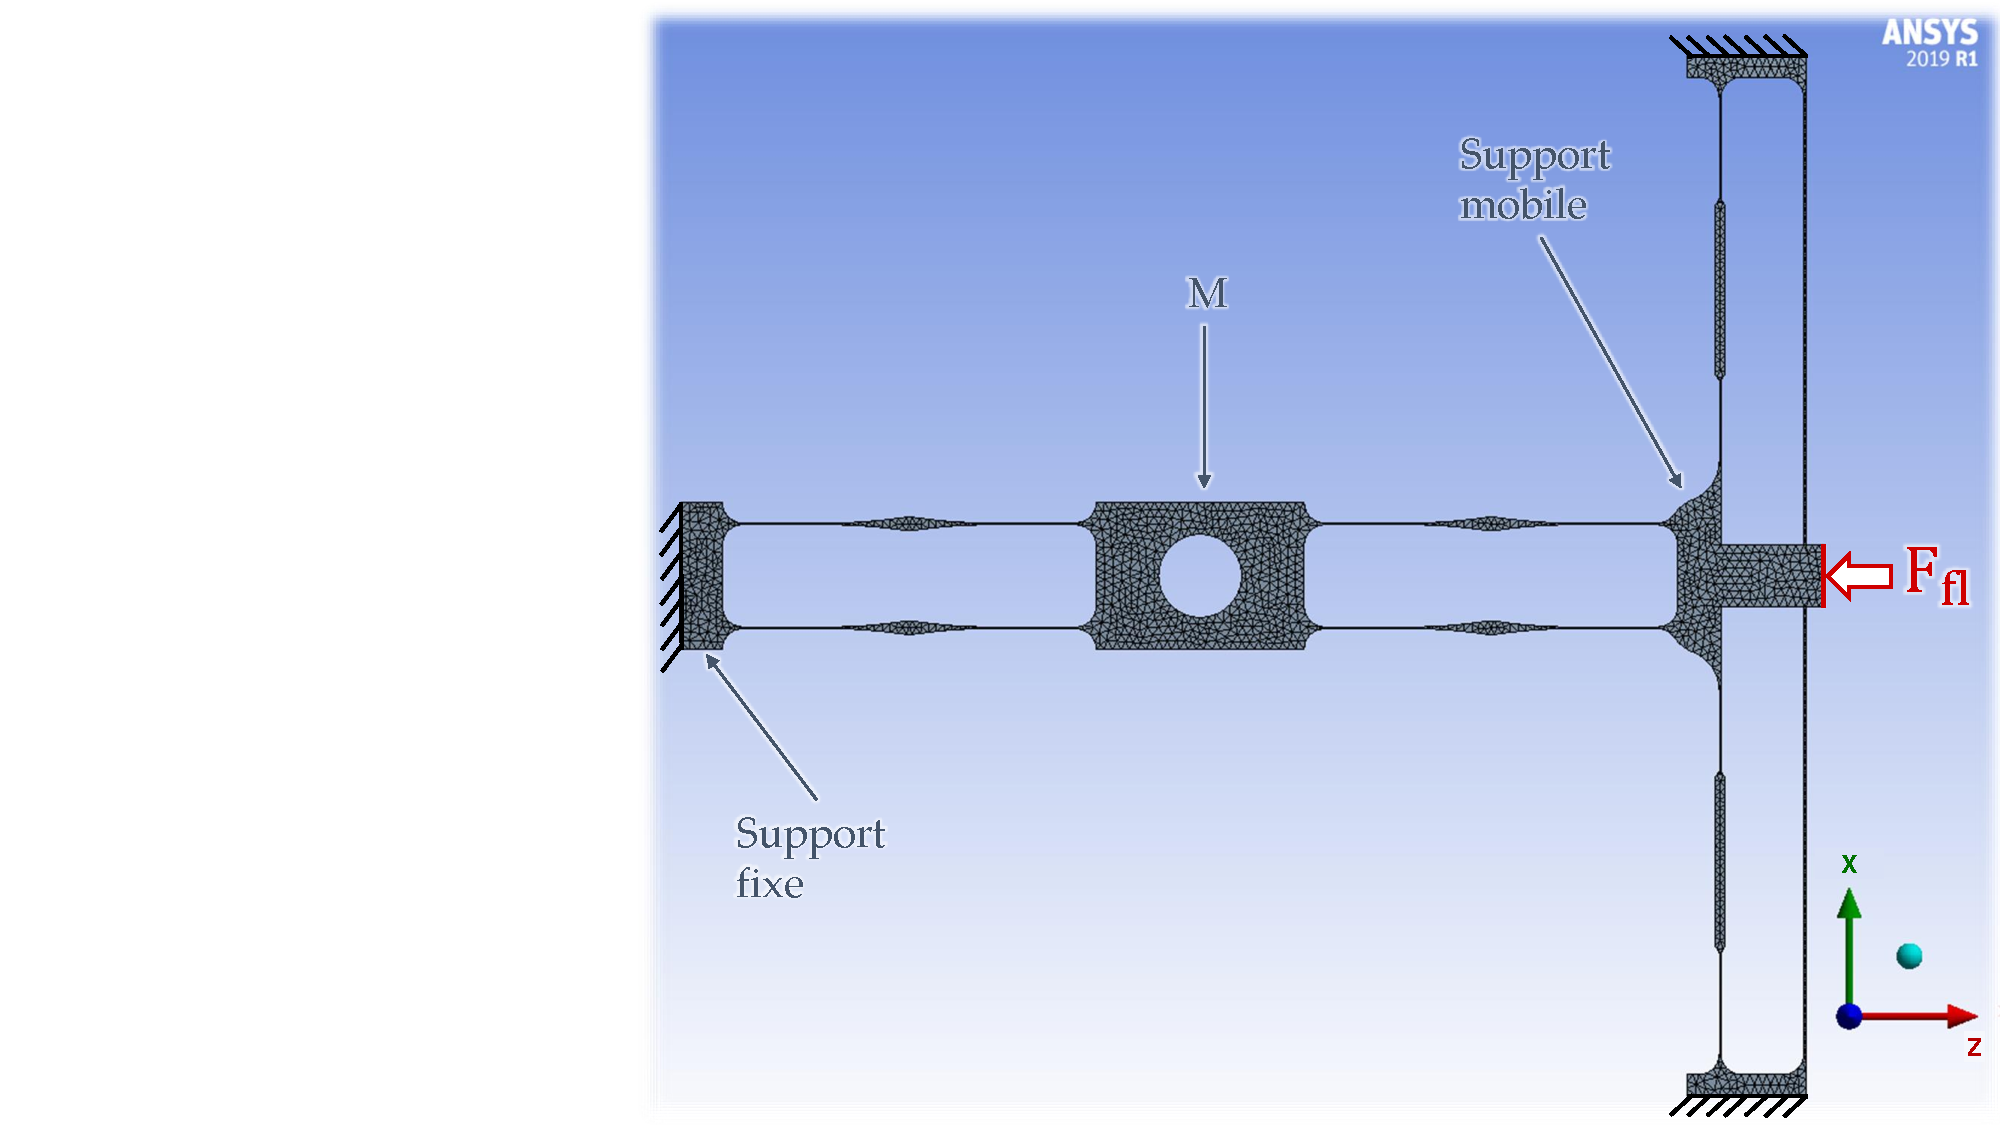
\includegraphics[trim={11cm 0cm 0cm 0cm},clip, width=0.8\textwidth]{../Chap3/Figure/EF_flambement_CI.pdf}
	\caption{Conditions initiales de l'étude de flambement EF de l'OB monobloc sur ANSYS}
	\label{fig:EF_flambement_CI}
\end{center}
\end{figure}
%%%%%%%%%%%

Pour cela, le comportement de l'OB sera considéré suivant les deux conceptions de lames, (SM) et (AM), respectivement sans et avec épaississement. Le modèle EF utilisé se base sur celui de l'étude statique présentée précédemment. Le schéma de la figure \ref{fig:EF_flambement_CI} montre alors les nouvelles conditions aux limites pour cette étude. La précontrainte de flambement induite par la vis micrométrique est modélisée par la force $F_{fl}=10$mN, appliquée à la surface se situant à l'extrémité droite du modèle. La résolution de l'étude de flambement en EF renseigne alors sur le coefficient multiplicateur de charge $m_{ch}$ à appliquer sur $F_{fl}=10mN$ afin de faire apparaître un mode de flambement spécifique. La force critique $F_{cfl}$ faisant apparaître un mode de flambement s'exprime alors par :
\begin{equation}
	F_{cfl}\ =\ m_{ch}\ F_{fl}
\label{eq:Force flambement EF}
\end{equation}

On considère seulement les résultats du mode de flambement utile et des quatre premiers modes de flambement secondaires. Les coefficients $m_{ch}$ respectifs à chaque mode sont présentés dans le tableau \ref{fig:EF_flambement_avec_et_sans_masselotte} pour les deux conceptions considérées. Le mode de flambement privilégié semble être le mode $utile$ pour chaque cas et se produit pour des valeurs de $m_{ch}$ quasiment identiques. L'épaississement local a par conséquent un effet négligeable sur l'apparition de ce mode. La force $F_{cfl}$ correspondant à la précontrainte est estimée pour le mode utile à $0.54$N pour la configuration SM et $0.61$N pour celle AM. Elle valide donc le critère d'infériorité par rapport à $F_{adm}$.	

En revanche, des différence sont notables entre les deux conceptions si on compare  $m_{ch}$ pour les modes de déformation secondaires suivant l'axe $\vec{x}$ illustrés sur la figure \ref{fig:EF_flambement_avec_et_sans_masselotte}. Les quatre premiers modes de flambement secondaires sollicités sur les deux conceptions sont les mêmes. Cependant, $F_{cfl}$ doit être trois fois plus importante pour induire des flambements locaux indésirables sur les LH (AM). L'épaississement local apporte donc une résistance structurelle trois fois plus importante face à l'apparition des modes de flambement indésirables. 

De plus, en combinant les équations \ref{eq:Force flambement EF} et \ref{fig:Fz(x0)} avec les valeurs du tableau \ref{tab:multiplicateur_de_charge_flambement}, on peut calculer le niveau de flambement maximal théorique $x_{0,max}$ de l'OB à vide avec l'équation \ref{x0_max}. Au delà de cette valeur de réglage pour l'OB seul, on verraient apparaître les modes indésirables dégradant $k_{sys}^2$. Le niveau de flambement maximal théorique pour les deux configurations est donné dans le tableau \ref{tab:x0max} pour garantir un $k_{sys}^2$ optimal avec les dimensions de lames du tableau \ref{tab:parametres_lames}.
%%%%%%%%%%%%%%%%%%%%%%%%%%%%%%%%%%%%	
\begin{table}[!htbp]
	\centering
%	\renewcommand{\arraystretch}{1}
		\begin{tabular}[t]{c|c|c|c|c|c|c|c|c|c|c|}
\cline{2-11} 
& \multicolumn{10}{c|}{\textbf{Mode de flambement}}\\
\cline{2-11} 
& \multicolumn{5}{c|}{\textbf{SM}} &  \multicolumn{5}{c|}{\textbf{AM}} \\
\cline{2-11} 
& Utile & a & b & c & d & Utile & e & f & g & h \\
\cline{2-11} \hline
\multicolumn{1}{|c|}{$m_{ch}$ [~~]} &
53.5 & 217.3	&	217.5	&	217.5	&	217.6	&
61.2 & 639.9	&	641.4	&	645		&	648.7 \\
\hline
		\end{tabular}
        \caption{Multiplicateur de charge nécessaire à l'apparition du mode de flambement pour $F_{fl} = 10$mN}
        \label{tab:multiplicateur_de_charge_flambement}
\end{table}        
%%%%%%%%%%%%%%%%%%%%%%%%%%%%%%%%%%%%
%%%%%%%%%%%
\begin{figure}[!htbp]
\begin{center}
    \captionsetup{justification=centering}
	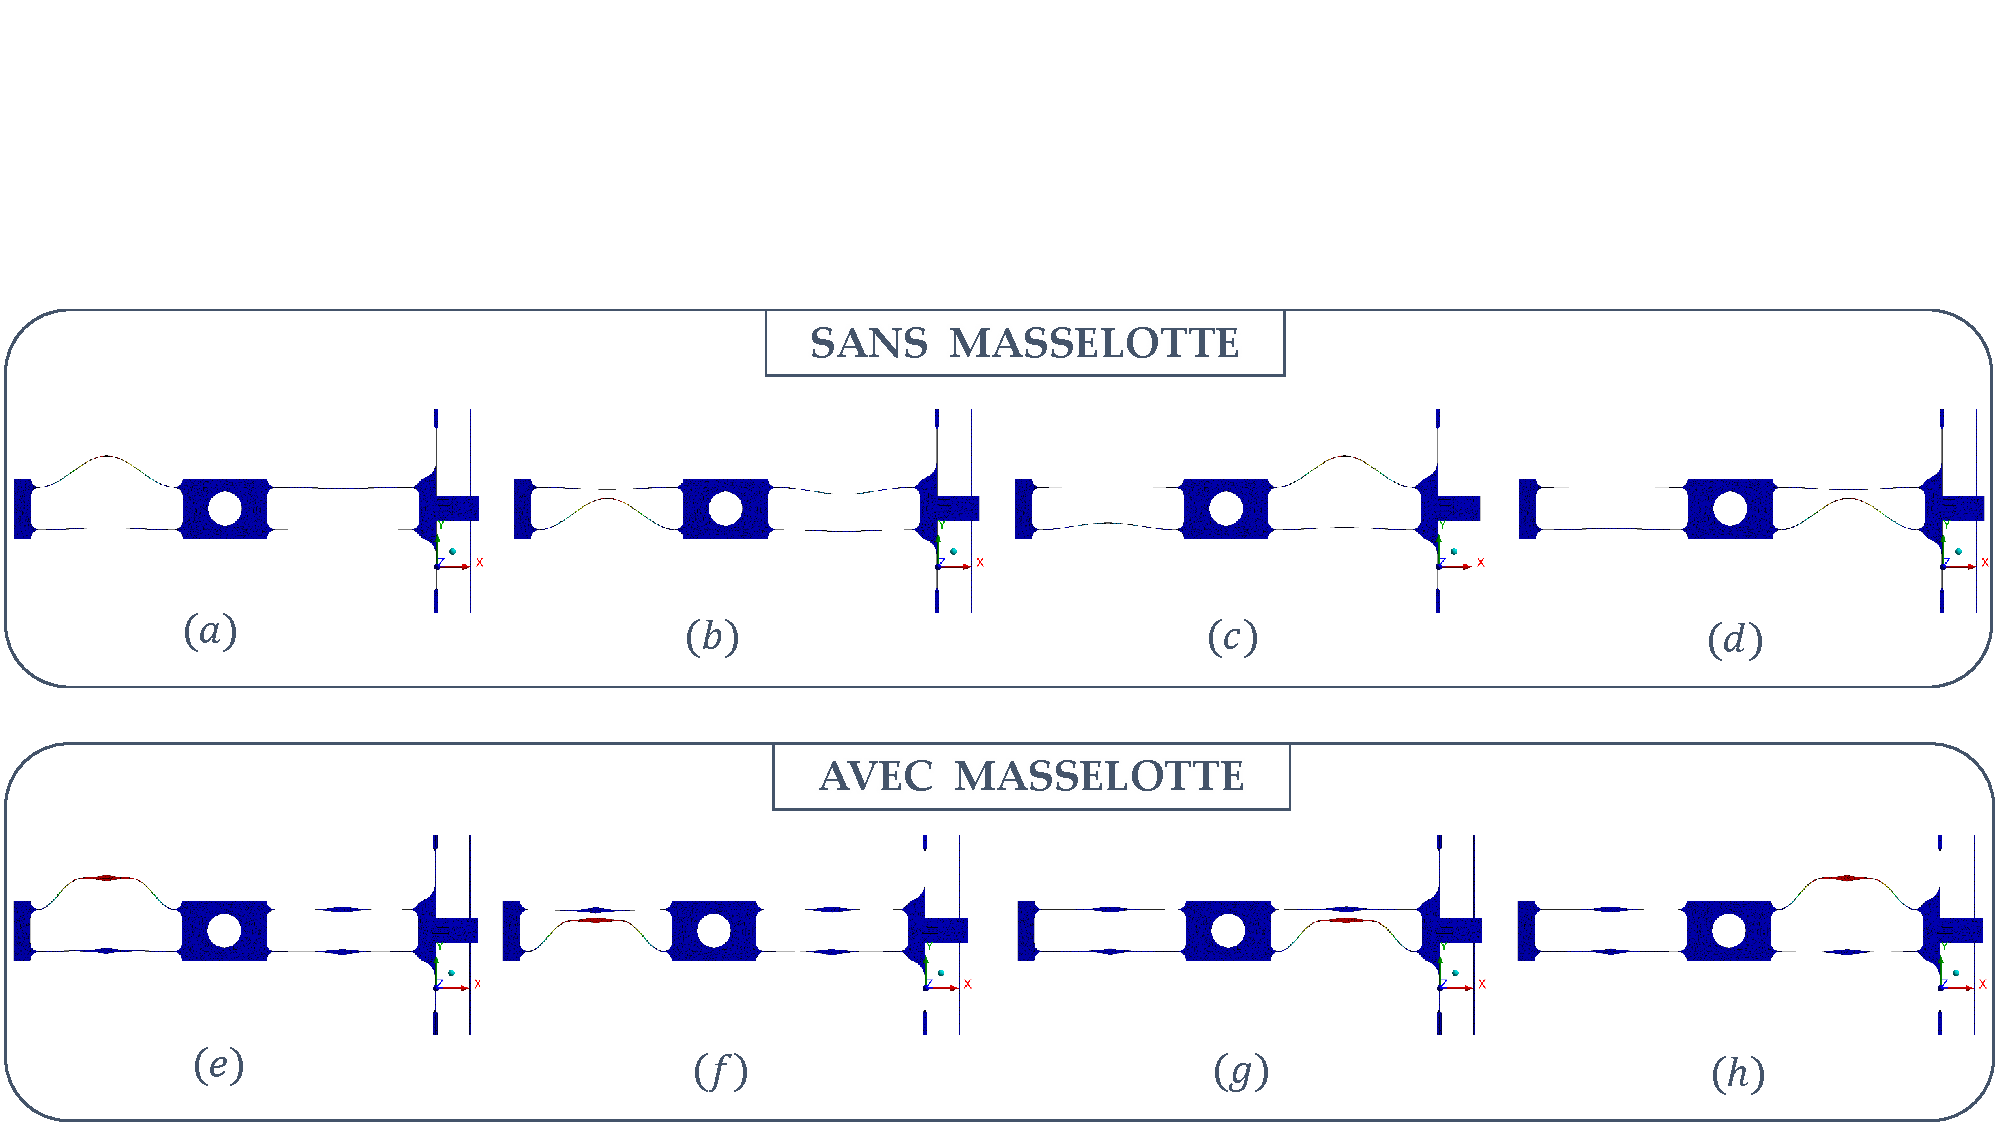
\includegraphics[trim={0cm 0cm 0cm 5cm},clip, width=\textwidth]{../Chap3/Figure/EF_flambement_avec_et_sans_masselotte.pdf}
	\caption{Illustration des 4 premiers modes de flambement indésirables pour les configurations de l'OB SM(a,b,c,d) et AM(e,f,g,h).}
	\label{fig:EF_flambement_avec_et_sans_masselotte}
\end{center}
\end{figure}
%%%%%%%%%%%
\begin{equation}
	x_{0,max} = \sqrt{\biggl(\dfrac{F_{cfl}}{2K} + L\biggr)^2 - L^2}
	\label{x0_max}
\end{equation}
%%%%%%%%%%%%%%%%%
\begin{table}[H]
	\centering
	\captionsetup{justification=centering}
	\rowcolors[]{2}{black!8}{}{
		\begin{tabular}{ c  c  }
			\rowcolor{blue!10}
			\rowcolor{blue!10}
			\toprule
			\textbf{Configuration} & \textbf{$x_{0,max}$} \\
			\midrule
			SM                     & 0.37mm               \\
			AM                     & 0.63mm               \\
			\bottomrule
		\end{tabular}}
	\caption{Niveau de flambement maximal à privilégier sur l'OB en fonction des conceptions des LFs}
	\label{tab:x0max}
\end{table}
%%%%%%%%%%%%%%%%%%%%%  

En conclusion, l'étude de flambement en EF valide le dimensionnement des LFs. De plus, la conception (AM) est à privilégier pour maximiser le $k_{sys}^2$ d'un convertisseur électromécanique suivant l'architecture d'OB considérée, en minimisant le risque d'apparition de mode de flambement secondaire.  
%/!\/!\/!\/!\/!\/!\/!\/!\/!\/!\/!\/!\/!\/!\/!\/!\/!\/!\/!\/!\/!\/!\/!\/!\%
\section{Dimensionnement des lames de guidage}
\label{sec:3.2:Dimensionnement des lames de guidage}
%/!\/!\/!\/!\/!\/!\/!\/!\/!\/!\/!\/!\/!\/!\/!\/!\/!\/!\/!\/!\/!\/!\/!\/!\%
    %/////////////////////////////////////////////
	\subsection{Cahier des charges}
	\label{subsec:3.2.2:Cahier des charges}
    %/////////////////////////////////////////////	
Les LGs doivent assurer la mise et le maintien en position du GPA, tout en lui évitant les rotations indésirables autour des axes $\vec{z}$ et $\vec{y}$. La LG ajoutée au montage ne jouera pas de rôle dans le bilan énergétique du convertisseur. Elle doit être assez rigide pour garantir la résistance en rotation autour de l'axe $z$ mais assez souple pour permettre à la vis micrométrique d'appliquer la précontrainte de flambement structurelle. Sa largeur a donc été estimée qualitativement à $0.1$mm et pourra être facilement modifiée si besoin.

Lorsque M se déplace d'une position stable vers l'autre, son énergie potentielle est en partie emmagasinée dans la coque du GPA et en partie dans la flexion de la LG usinée. L'énergie stockée dans la LG ne peut être convertie par le GPA. Afin de maximiser le coefficient de couplage électromécanique du système, il faut s'assurer que les efforts de traction/compression suivant l'axe $\vec{z}$ sont majoritairement repris par le GPA. Cela revient à vérifier que la raideur $K_{LG}$ de la LG usinée est négligeable devant la raideur $K$ du GPA.
    %/////////////////////////////////////////////
	\subsection{Approche analytique}
	\label{subsec:3.2.1:Approche analytique LG}
    %/////////////////////////////////////////////
Les LFs transmettent les efforts de compression depuis la masse vers le GPA. Par conséquent, elles peuvent être modélisés par des raideurs en série avec ce-dernier. La LG usinée, en revanche, absorbe les efforts transmis depuis les LFs, de la même manière que le GPA. Elle peut donc être modélisée par une raideur en parallèle avec celle du GPA. La raideur équivalente du système composé de l'OB et du GPA peut alors être exprimée en fonction des raideurs des différents éléments, à travers l'équation \ref{eq:Keq}.
\begin{equation}
	K_{eq} = \dfrac{K_{LF}(K + K_{LG})}{K_{LF}+ K + K_{LG}}
	\label{eq:Keq}
\end{equation}
$K_{eq}$ représente la raideur "vue" du point de vue de la masse, sur l'axe $\vec{z}$. Avec $K_{LF}$ la raideur en compression des quatres LFs, $K_{LG}$ la raideur en flexion de la LG usinée et $K$ la raideur du GPA. Le coefficient de couplage électromécanique $k^2_{sys}$ du convertisseur électromécanique peut alors être exprimé en fonction la raideur équivalente du système dans l'équation \ref{eq:k^2_eq}. Où $\alpha$ et $C_0$ sont les paramètres électriques du GPA, définis dans le tableau \ref{tab:parametres}.
\begin{equation}
	k^2_{sys} = \dfrac{\alpha^2 }{\alpha^2 + K_{eq}C_0}
	\label{eq:k^2_eq}
\end{equation}
Afin de maximiser $k^2_{sys}$, il faut $K_{eq}\approx K$. Pour de satisfaire cette égalité, il faut que $K_{LF}>>K$ pour une bonne transmissions des efforts depuis l'OB vers le GPA. Ceci a été vérifié dans la sous-section \ref{sec:3.3.1_Limite structurelle et précontrainte de flambement}. De plus, il faut $K>>K_{LG}$ pour que les efforts soient majoritairement absorbés par le GPA. La modélisation qui suit permettra de vérifier cette dernière hypothèse.
 
Les épaississements locaux n'ont pas d'influence significative sur la raideur en rotation des LFs d'après les observations faites dans la section précédente. Nous allons donc modéliser la double portion de LG usinée comme une seule LG de largeur $L_v$ constante, d'épaisseur $e$ et longueur $l_v$. 
%%%%%%%%%%%
\begin{figure}[!htbp]
\begin{center}
    \captionsetup{justification=centering}
	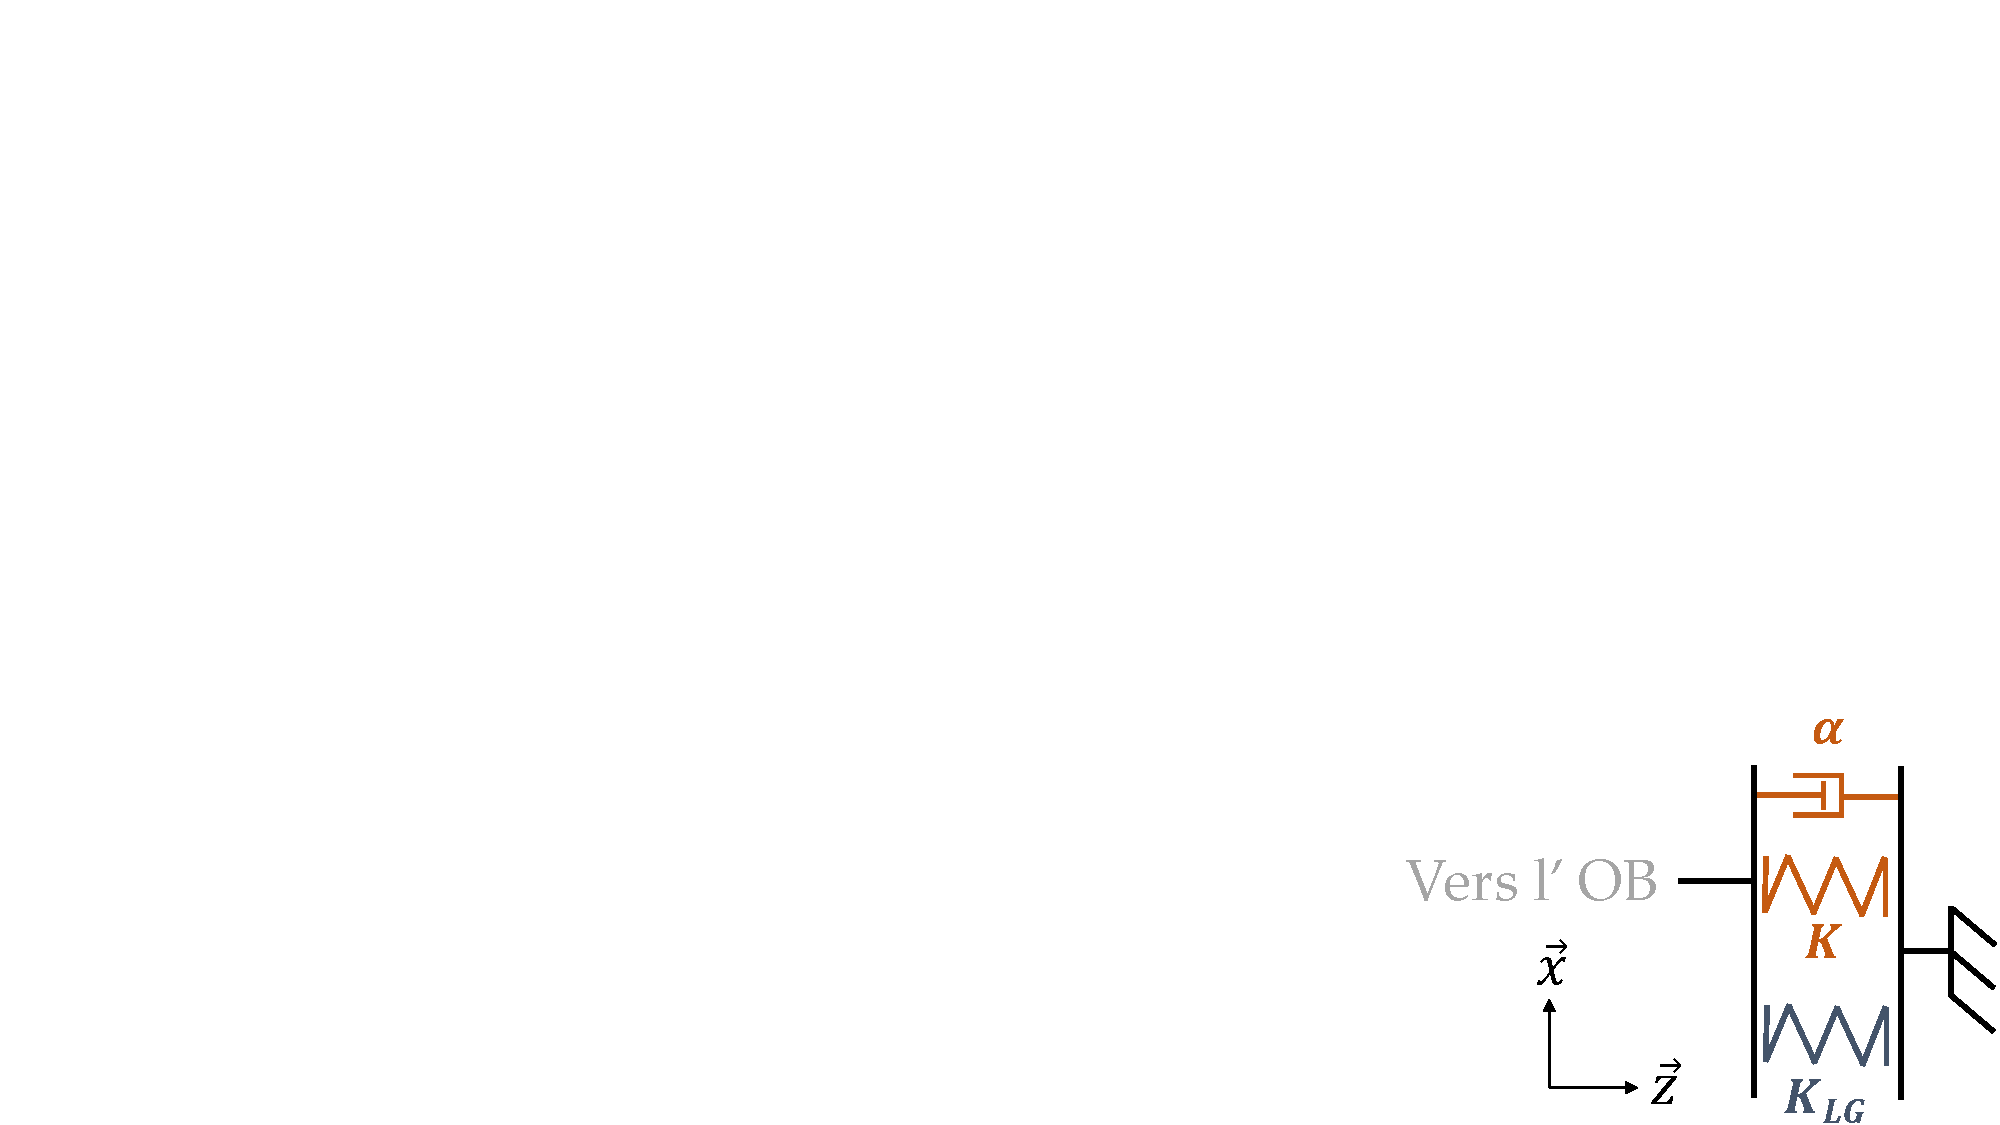
\includegraphics[trim={23.5cm 0cm 0cm 12cm}, clip,width=0.3\textwidth]{../Chap3/Figure/KGPA_Kv2.pdf}
	\caption{Modélisation statique du GPA avec la LG usinée}
	\label{fig:KGPA_Kv}
\end{center}	
\end{figure}
%%%%%%%%%%%
%%%%%%%%%%%
\begin{figure}[!htbp]
\begin{center}
    \captionsetup{justification=centering}
	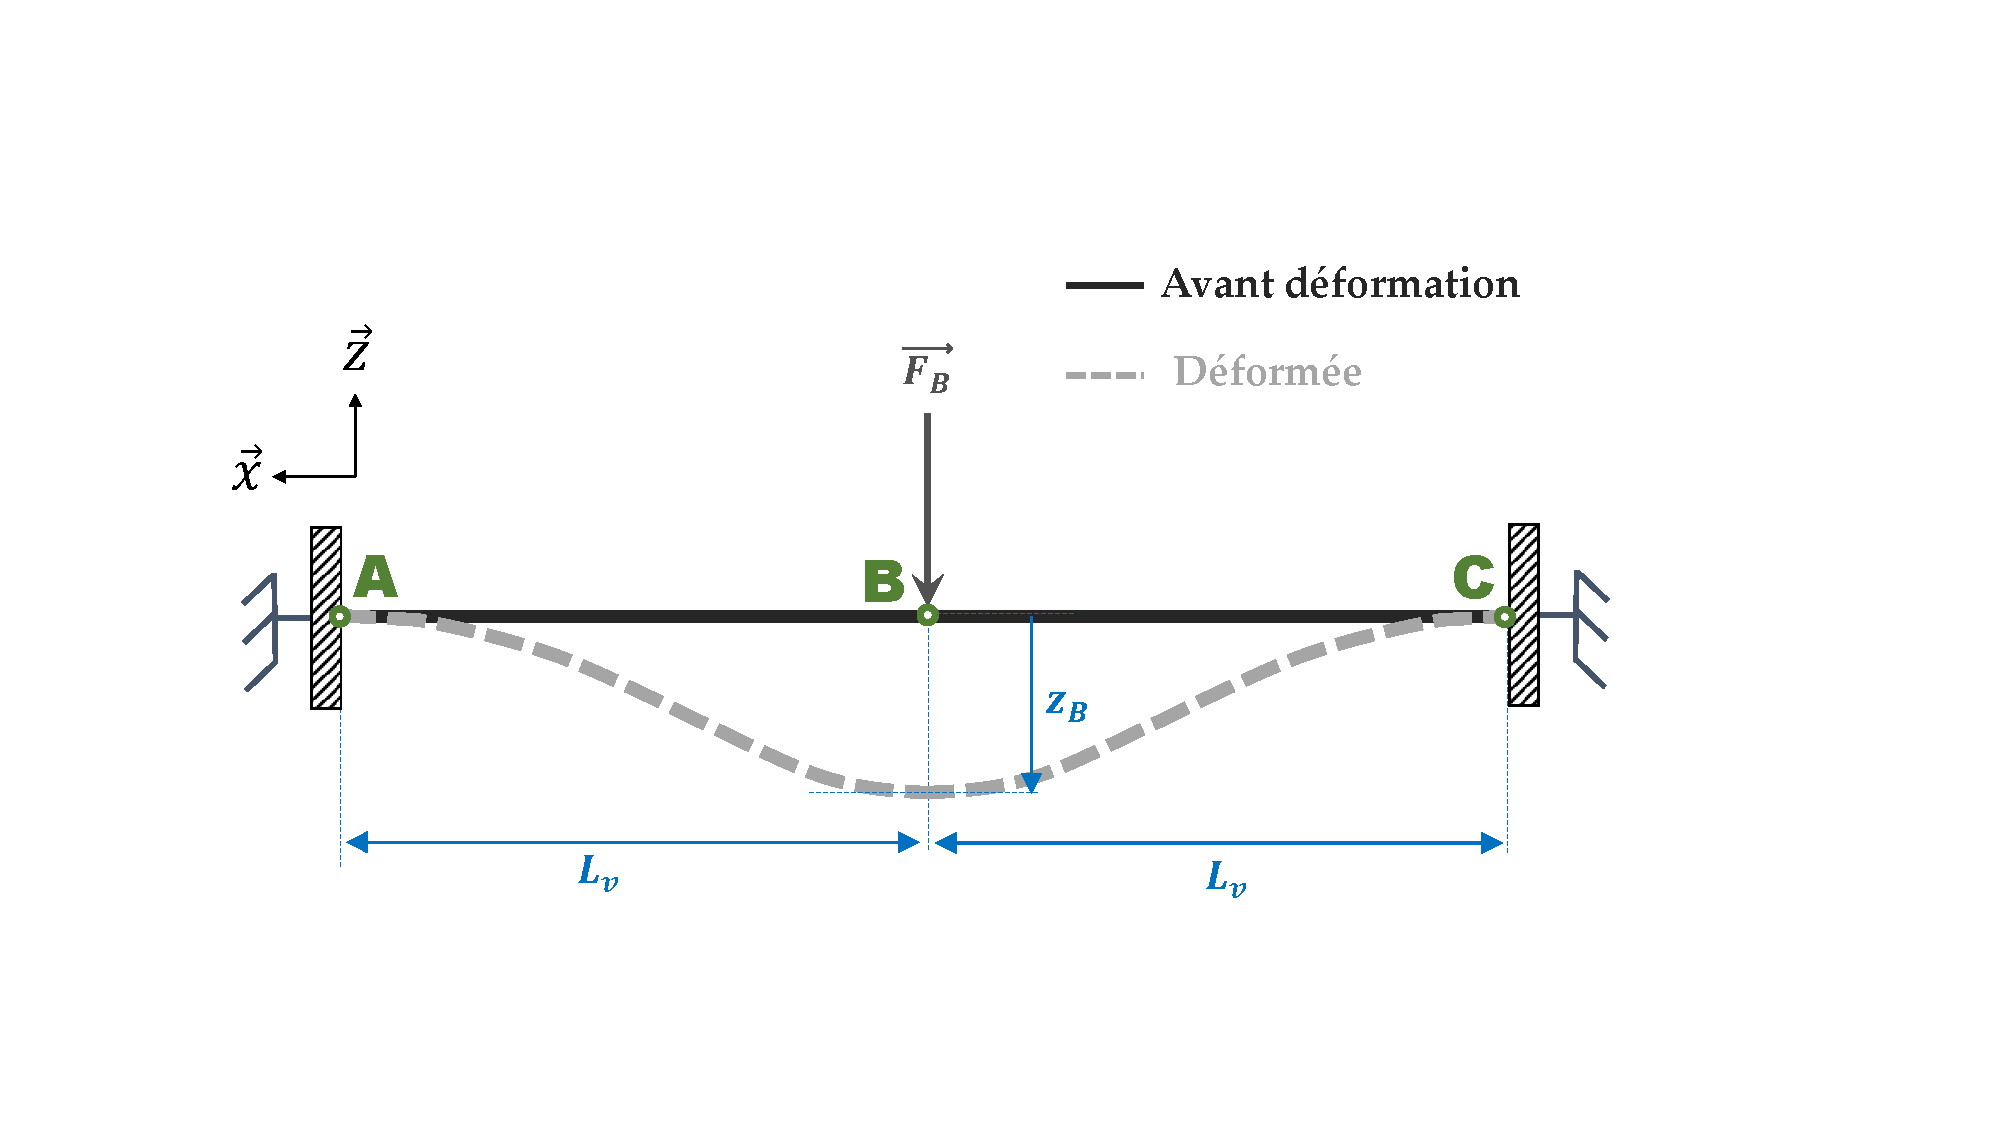
\includegraphics[trim={4cm 3cm 6.5cm 4.5cm},clip, width=0.7\textwidth]{../Chap3/Figure/Kv_modele2.pdf}
	\caption{Schéma de la poutre de guidage sous sollicitations}
	\label{fig:Kv_modele}
\end{center}	
\end{figure}
%%%%%%%%%%%

Sur l'architecture actuelle, la déformation de la LG usinée s'apparente au cas standard d'une poutre bi-encastrée subissant un effort normal en son centre. La figure \ref{fig:Kv_modele} schématise cette configuration d'étude avec $F_B$ l'effort transmis depuis l'OB. La rigidité d'une LG dans cette configuration peut alors être définie comme suit :
\begin{equation}
K_{LG}\ =\ \frac{F_B}{z_B}
\label{eq:def_Kv}
\end{equation}

Où $z_B$ est la flèche de la poutre en B. Celle-ci peut être exprimée, pour ce cas de sollicitation, par l'équation \ref{eq:fleche_encastré-encastré} \cite{Courbon1988}. Où $I_v$ est le moment quadratique de la LG usinée suivant l'axe $\vec{y}$, exprimé par l'équation \ref{eq:Iv moment quadratique LG}.
\begin{equation}
z_B\ =\ \frac{F_B\ {(2L_v)}^3}{192\ E\ I_v}
\label{eq:fleche_encastré-encastré}
\end{equation}
\begin{equation}
	I_v = \dfrac{e\ {l_v}^3}{12}
\label{eq:Iv moment quadratique LG}
\end{equation}

$K_{LG}$ peut donc être reformulée en combinant les équations \ref{eq:def_Kv} et \ref{eq:fleche_encastré-encastré}, pour donner l'équation \ref{eq:K_{LG} definition poutre bi encastree}.
\begin{equation}
K_{LG}\ =\ \frac{2\ E\ I_v}{{l_v}^3}
\label{eq:K_{LG} definition poutre bi encastree}
\end{equation}

Enfin, en considérant les équations \ref{eq:K_{LG} definition poutre bi encastree} et \ref{eq:Iv moment quadratique LG}, on peut établir la relation entre la rigidité de la LG usinée et ses paramètres géométriques et matériau, à travers l'équation \ref{eq:Kv en fonction des paramètres de LG}.
\begin{equation}
	K_{LG} = \dfrac{2Ee{l_v}^3}{{L_v}^3}
\label{eq:Kv en fonction des paramètres de LG}
\end{equation}

On doit alors vérifier la condition suivante pour le bon fonctionnement du système:
\begin{equation}
K >> K_{LG}
\label{eq:rapport_K/Kv}
\end{equation}

Avec les valeurs des paramètres définies dans le tableau \ref{tab:parametres_lames}, et le choix du modèle de transducteur APA50XS du fournisseur Cedrat Technologies, on vérifie alors que :
\begin{equation}
\frac{K_{LG}}{K} = \frac{4\cdot 10^{-2}}{256\cdot 10^3}\approx 1.6\cdot 10^{-7}
\end{equation}

La raideur en flexion de la LG usinée est bien négligeable devant celle du GPA. Son influence sur le coefficient de couplage électromécanique du système sera donc négligeable. On valide par là le dimensionnement de la LG usinée.
%/!\/!\/!\/!\/!\/!\/!\/!\/!\/!\/!\/!\/!\/!\/!\/!\/!\/!\/!\/!\/!\/!\/!\/!\%
\section{Caractérisations expérimentales du convertisseur électromécanique}
\label{sec:3.3}
%/!\/!\/!\/!\/!\/!\/!\/!\/!\/!\/!\/!\/!\/!\/!\/!\/!\/!\/!\/!\/!\/!\/!\/!\%
Cette section présente le banc de test visant à mener les caractérisations électromécaniques de l'ensemble OB+GPA. Il sera utilisé pour corréler le comportement dynamique de l'OB, ainsi que le comportement électrique du GPA, avec ceux simulés pour le pré-dimensionnement (sec. \ref{subsec:2.5.3:Simulation et resultats}).
    %/////////////////////////////////////////////
	\subsection{Présentation du banc de caractérisation}
    %/////////////////////////////////////////////
Le banc de caractérisation visant à valider expérimentalement le modèle du convertisseur électromagnétique développé dans le chapitre précédent est présenté sur la figure \ref{fig:BDT_OB+GPA}. Il se compose notamment de l'assemblage des éléments suivants:
\begin{itemize}[label=$\circ$]
	\item Assemblage OB monobloc avec GPA.
	\item Système du réglage de flambement constitué d'une vis micrométrique montée en série avec un roulement.
	\item Système d'actionnement hydraulique constitué de deux PHs.
	\item Un capteur de déplacement laser Panasonic HL-G103.
	\item Deux capteurs de déplacement fibre optique Philtech RC63.
\end{itemize}
%%%%%%%%%%%
\begin{figure}[!htbp]
\begin{center}
    \captionsetup{justification=centering}
	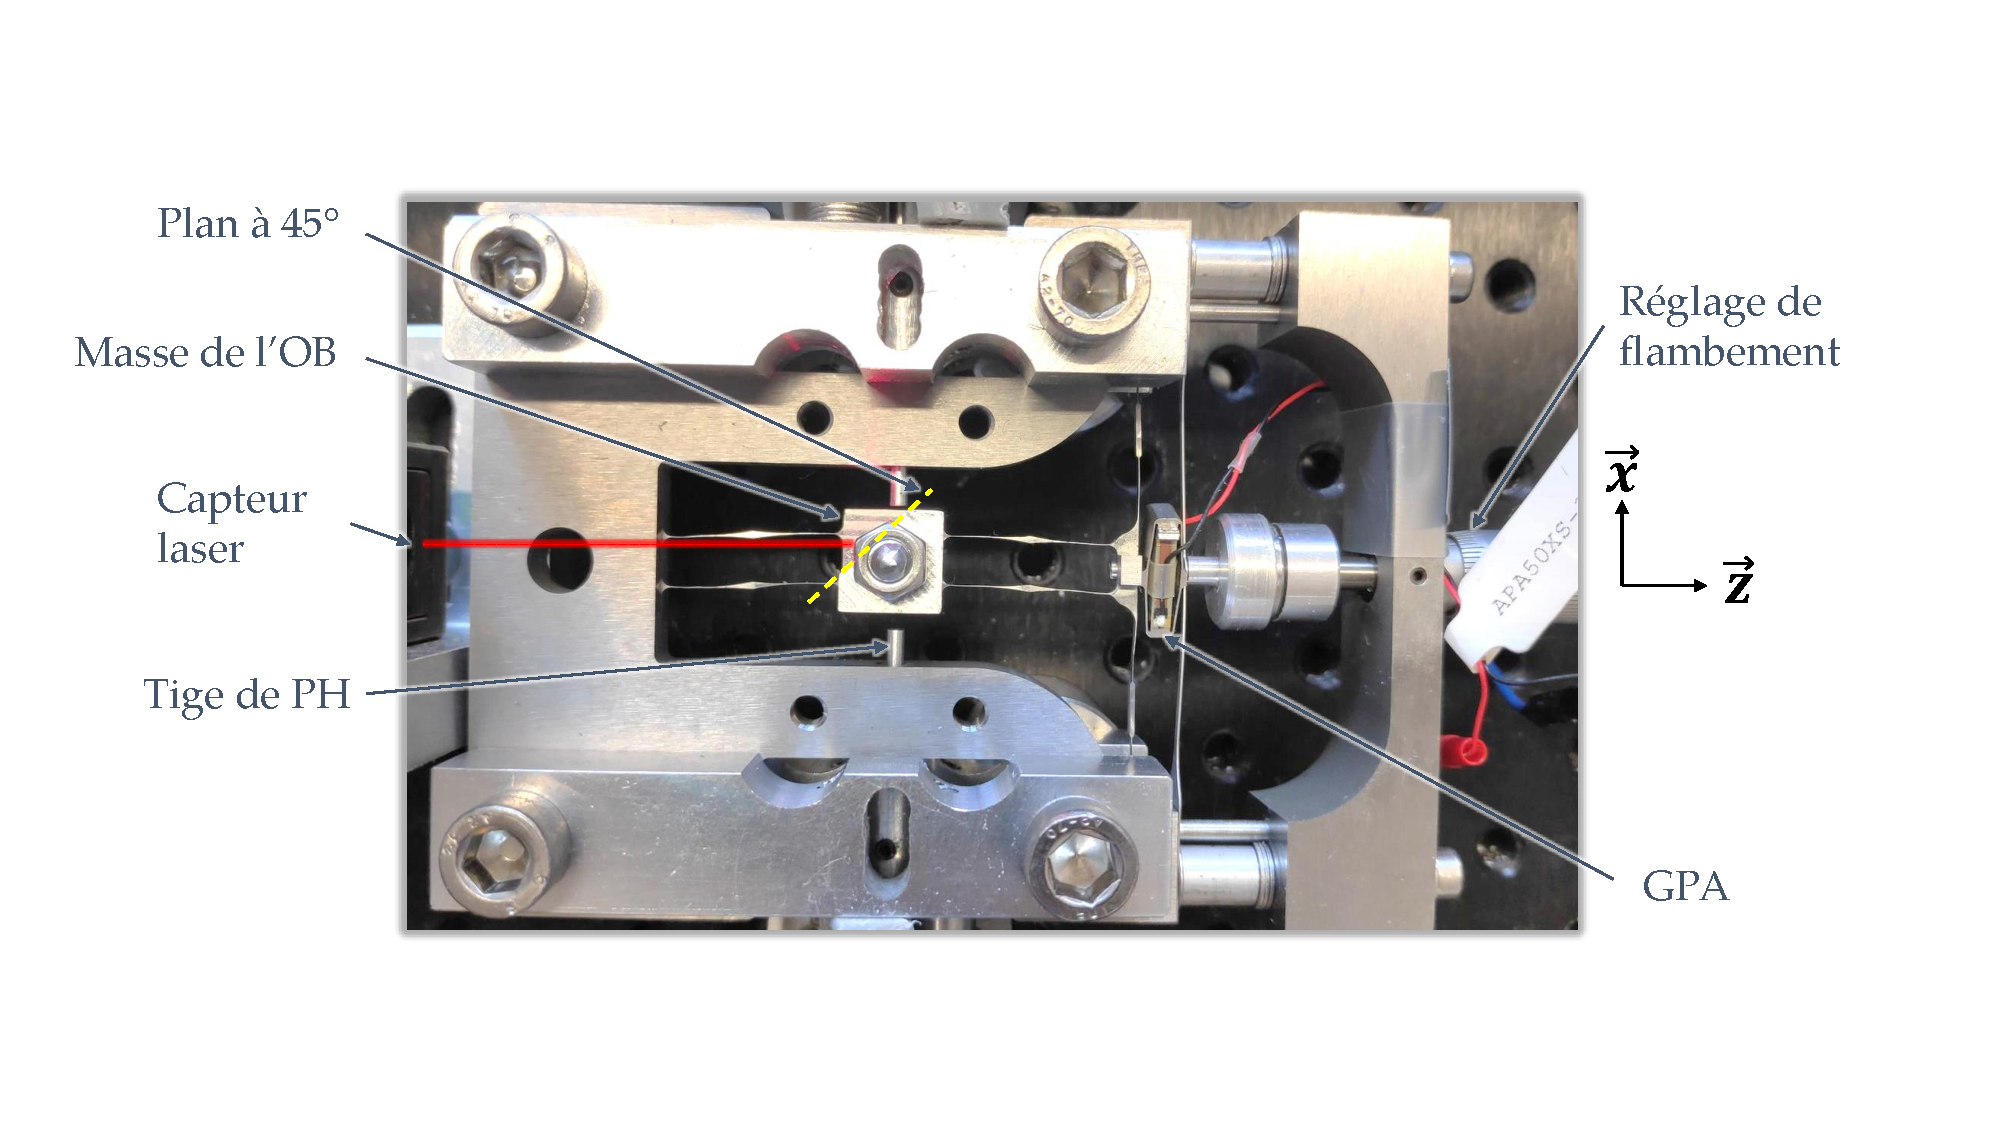
\includegraphics[trim={0.5cm 3cm 2cm 2.5cm},clip, width=0.9\textwidth]{../Chap3/Figure/BDT_OB+GPA.pdf}
	\caption{Vue de face de GPA et l'OB monobloc sur le banc de caractérisation électromécanique}
	\label{fig:BDT_OB+GPA}
\end{center}
\end{figure}
%%%%%%%%%%%		
%%%%%%%%%%%
\begin{figure}[!htbp]
\begin{center}
    \captionsetup{justification=centering}
	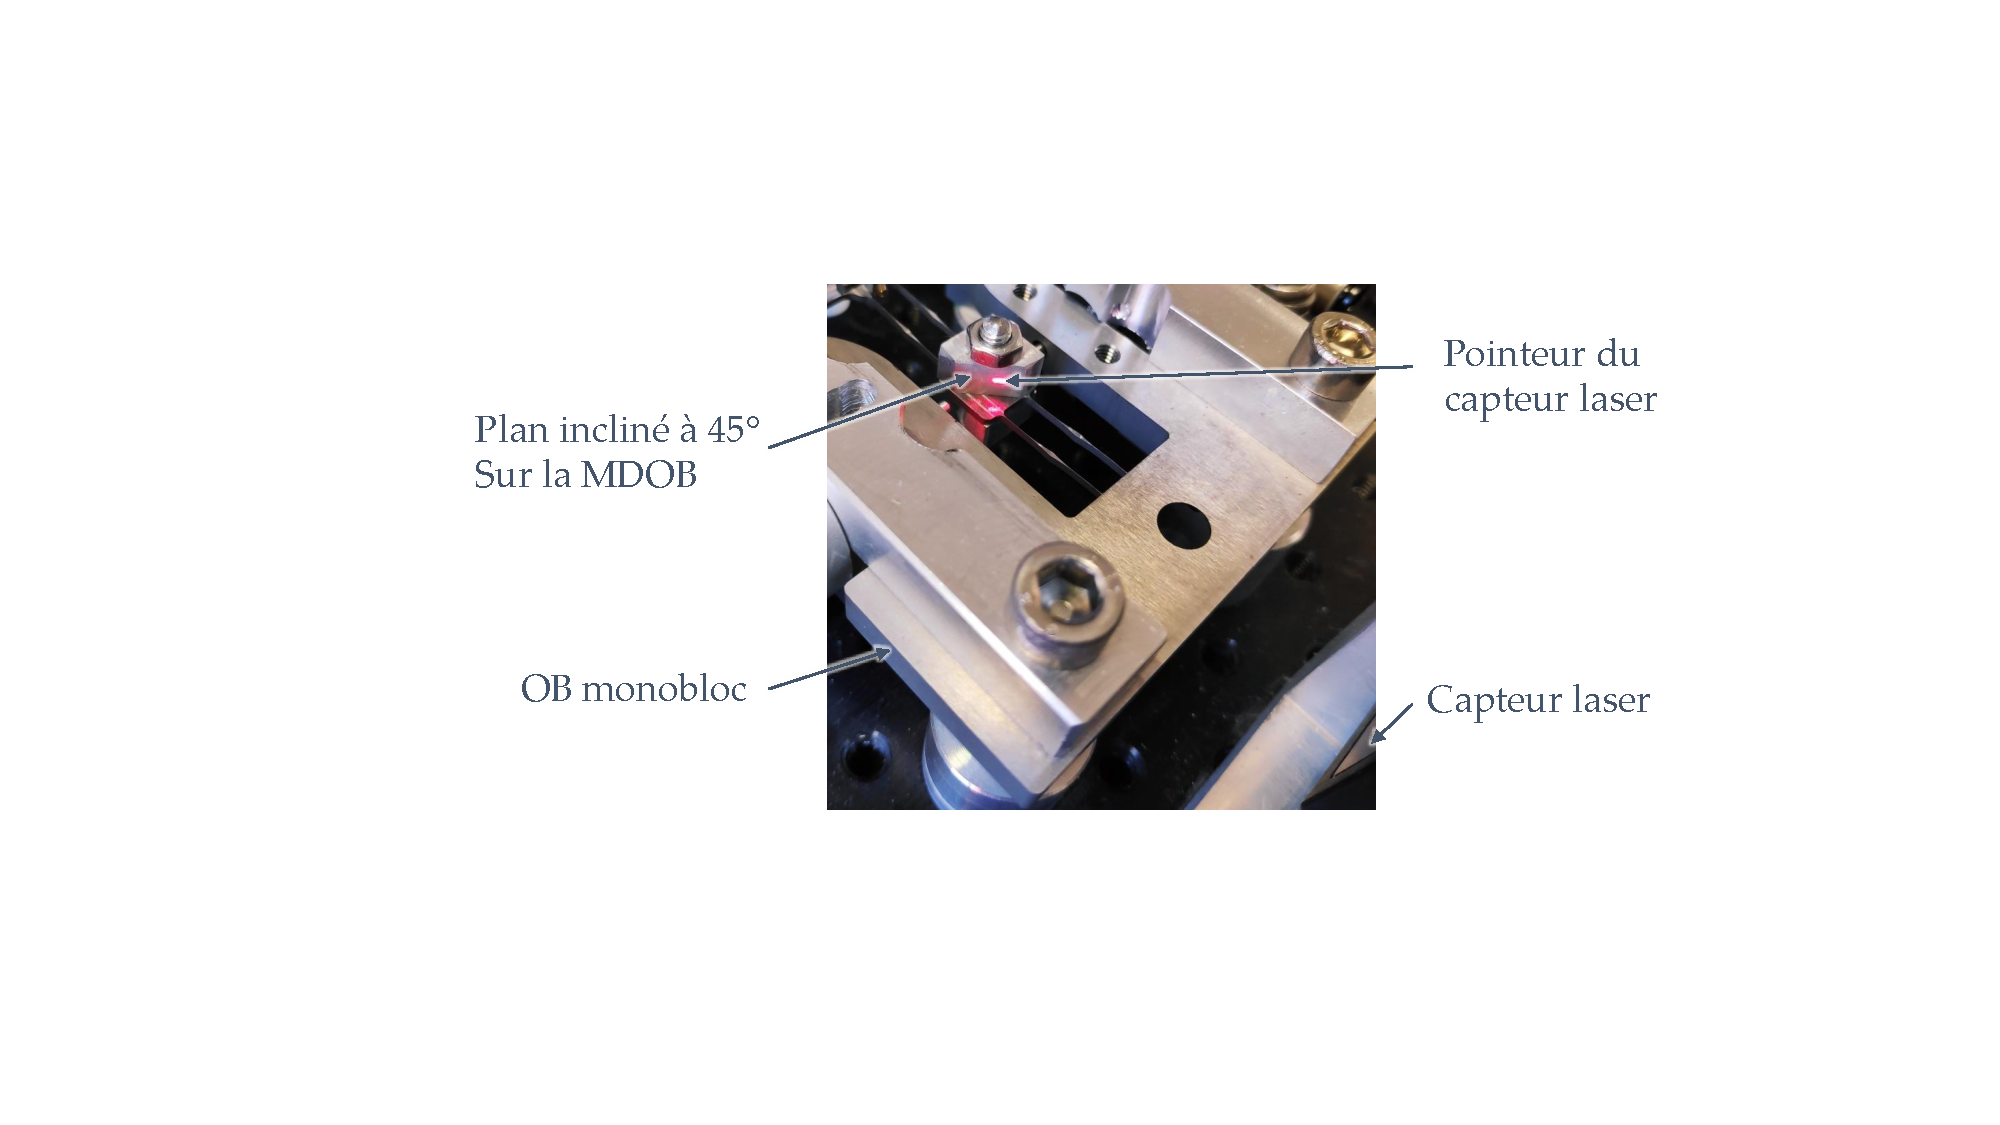
\includegraphics[trim={8cm 5cm 5.5cm 5cm},clip, width=0.7\textwidth]{../Chap3/Figure/BDT_detail_plan45.pdf}
	\caption{Détail sur le plan à 45° monté sur M pour le suivi en déplacement}
	\label{fig:BDT_detail_plan45}
\end{center}
\end{figure}
%%%%%%%%%%%	

La vis micrométrique permet le réglage du niveau de flambement de l'OB par un mouvement hélicoïdal qui déplace le GPA suivant l'axe $\vec{z}$. L'intégration du roulement en série permet alors de découpler la rotation entre la vis et le GPA. Ce découplage permet en effet d'éviter la génération de torsion sur la structure, suivant l'axe $\vec{z}$, lorsque la vis tourne.

Le capteur HL-G103 vise un plan à 45°, qui a été usiné sur un lest monté sur M pour mesurer son déplacement. Une vue de cet élément est présentée sur la figure \ref{fig:BDT_detail_plan45}. Il est assemblé sur la masse centrale au travers d'une tige filetée qu'on vient serrer de part et d'autre avec deux écrous. Son montage est réalisée de façon symétrique, par rapport au plan de face, avec une pièce identique pour que le centre de gravité de la masse centrale se trouve sur l'axe de la tige filetée. Le serrage des écrous a été réalisé de façon symétrique afin de minimiser les contraintes de torsion sur les LFs. Les capteurs RC63 visent une surface de silicium avec un polissage miroir pour une meilleure réflexion du signal de mesure. La plaque réfléchissante est alors montée sur un axe relié aux tiges de PH de façon à mesurer leurs déplacements respectifs. La figure \ref{fig:BDT_detail_capteur_RC63} montre le détail de la configuration de mesure de la position pour un PH.
%%%%%%%%%%%
\begin{figure}[!htbp]
\begin{center}
    \captionsetup{justification=centering}
	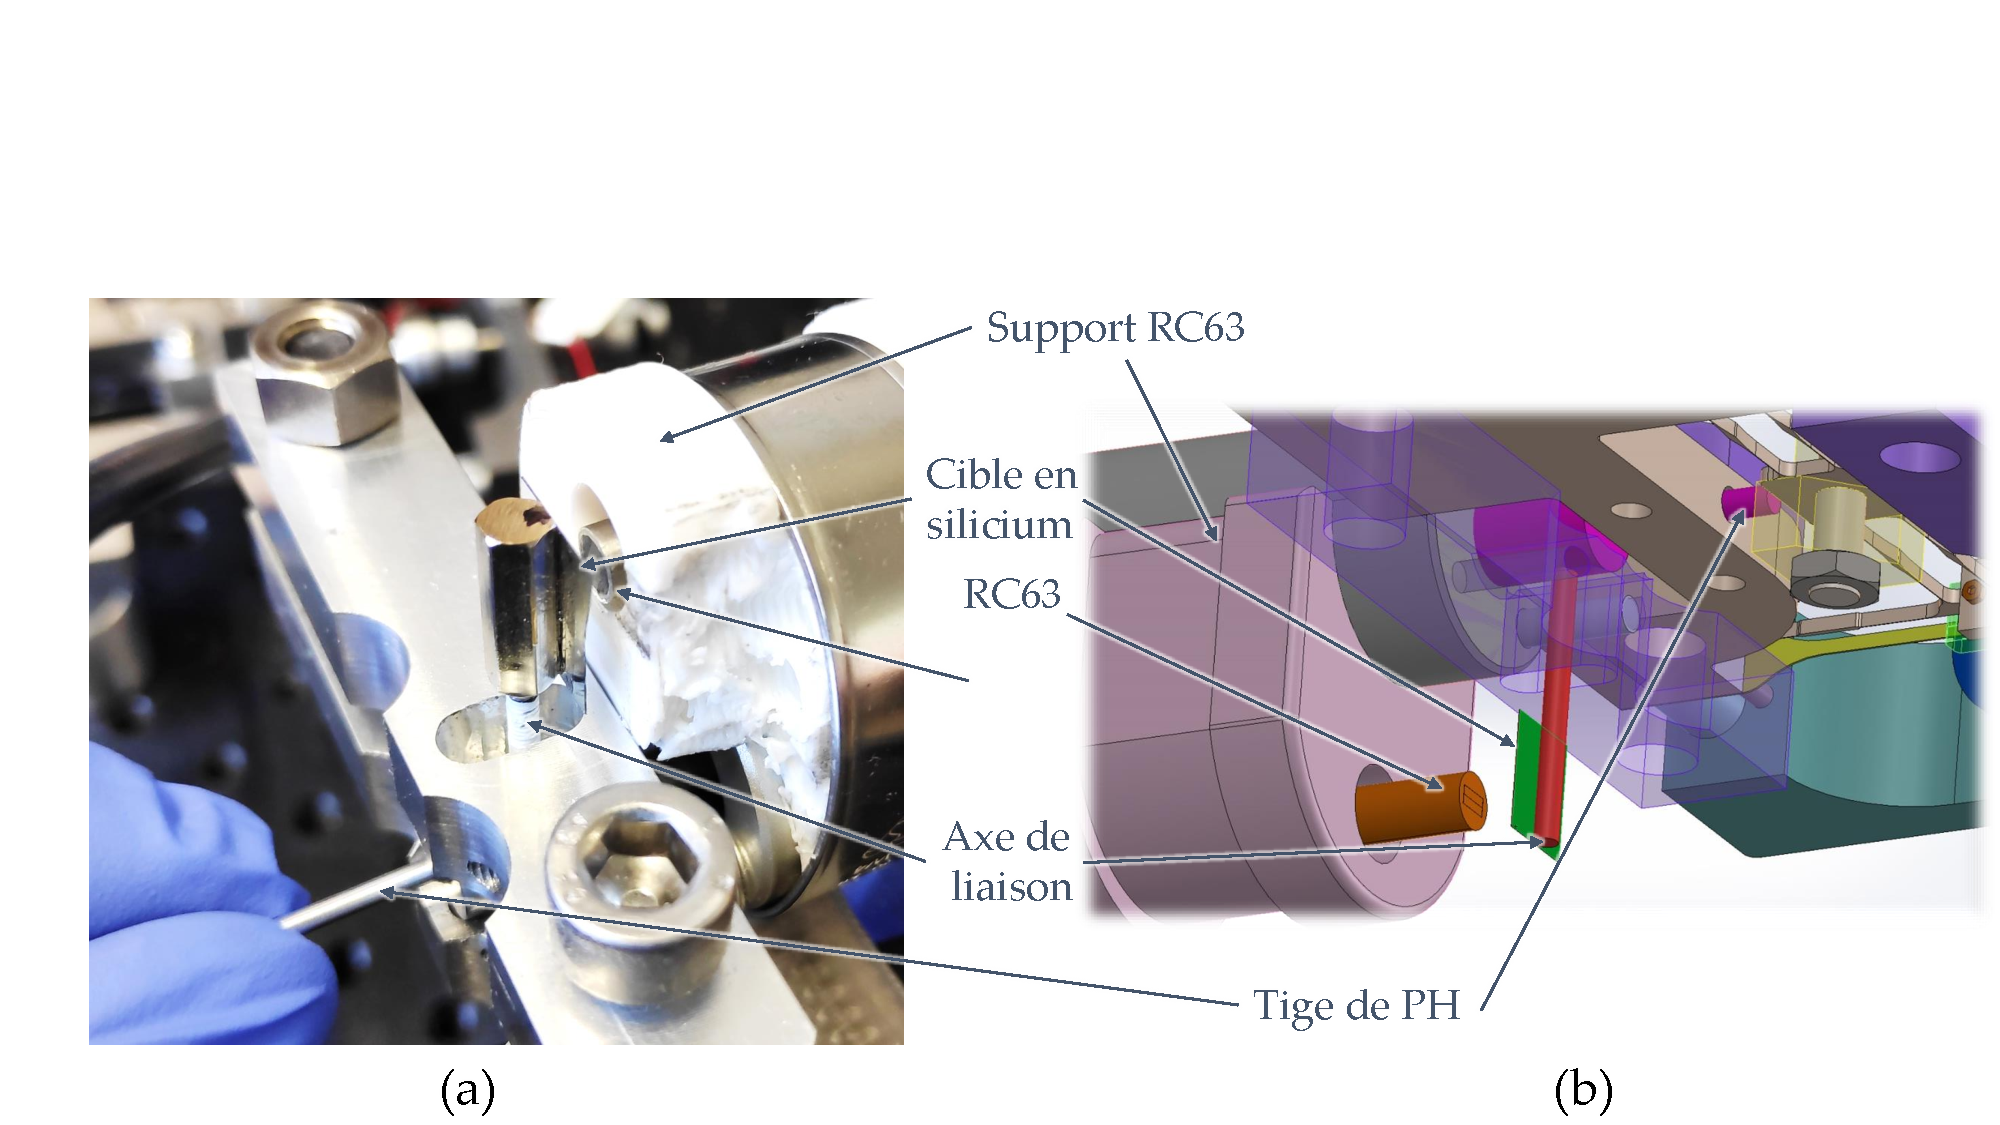
\includegraphics[trim={1.5cm 0cm 0cm 3cm},clip, width=\textwidth]{../Chap3/Figure/BDT_detail_capteur_RC63_2.pdf}
	\caption{(a) Image du montage du système de mesure du déplacement d'un PH. (b) Système de mesure du déplacement d'un PH intégré au banc de test}
	\label{fig:BDT_detail_capteur_RC63}
\end{center}
\end{figure}
%%%%%%%%%%%			

L'assemblage est surélevé à l'aide de quatre plots en aluminium, percés et traversés par les quatre vis M6 à tête creuse hexagonale qu'on aperçoit sur la figure \ref{fig:BDT_detail_plan45}. Deux des plots sont visibles sur la figure \ref{fig:BDT_detail_plan45}. La surélévation est nécessaire pour tenir compte de l'encombrement de la masse ajoutée avec la tige filetée traversante, de  l'instrumentation, ainsi que du corps des pistons. Les défauts de planéité sur les pièces usinées peuvent engendrer une déformation du montage lors du serrage des quatre vis et ainsi introduire une asymétrie dans le comportement de l'OB. Afin de minimiser ce phénomène, le couple de serrage des quatre vis a été limité à $25Nm$.

La puissance électrique générée par le GPA est dissipée dans une résistance de charge $R_{ch}$. Si $k^2_{sys}$ est modéré ($k^2_{sys}Q<2$), la résistance de charge peut être calculée à partir de la fréquence d'oscillation de l'OB et de la capacité interne du générateur, avec l'équation \ref{eq:Rch definition}, afin de maximiser la densité de puissance du générateur \cite{Lefeuvre2005}.
\begin{equation}
	R_{ch} = \frac{1}{C_0\ \omega_0}
	\label{eq:Rch definition}
\end{equation}
Le capteur de position laser, ainsi que la tension aux bornes du GPA sont reliés à une carte d'acquisition NI-USB 6212 qui est interfacée par LabVIEW sur un ordinateur.

La fabrication de l'OB monobloc a été réalisée avec une précision à $\pm5$µm, dans le respect de notre cahier des charges. Néanmoins après analyse optique au microscope, on s'aperçoit que la planéité des lames n'a pas été assurée lors de la fabrication. La figure \ref{fig:BDT_defauts_OB} met en évidence les défauts de fabrication au niveau des lames de l'OB monobloc. Les fortes ondulations au niveau de la LG usinée peuvent introduire une asymétrie entre les deux positions stables de l'oscillateur. La présence de la LG ajoutée au montage permettra de minimiser ce défaut en imposant l'alignement avec les goupilles de centrage visibles sur la figure \ref{fig:moboloc+GPA}.
%%%%%%%%%%%
\begin{figure}[!htbp]
\begin{center}
    \captionsetup{justification=centering}
	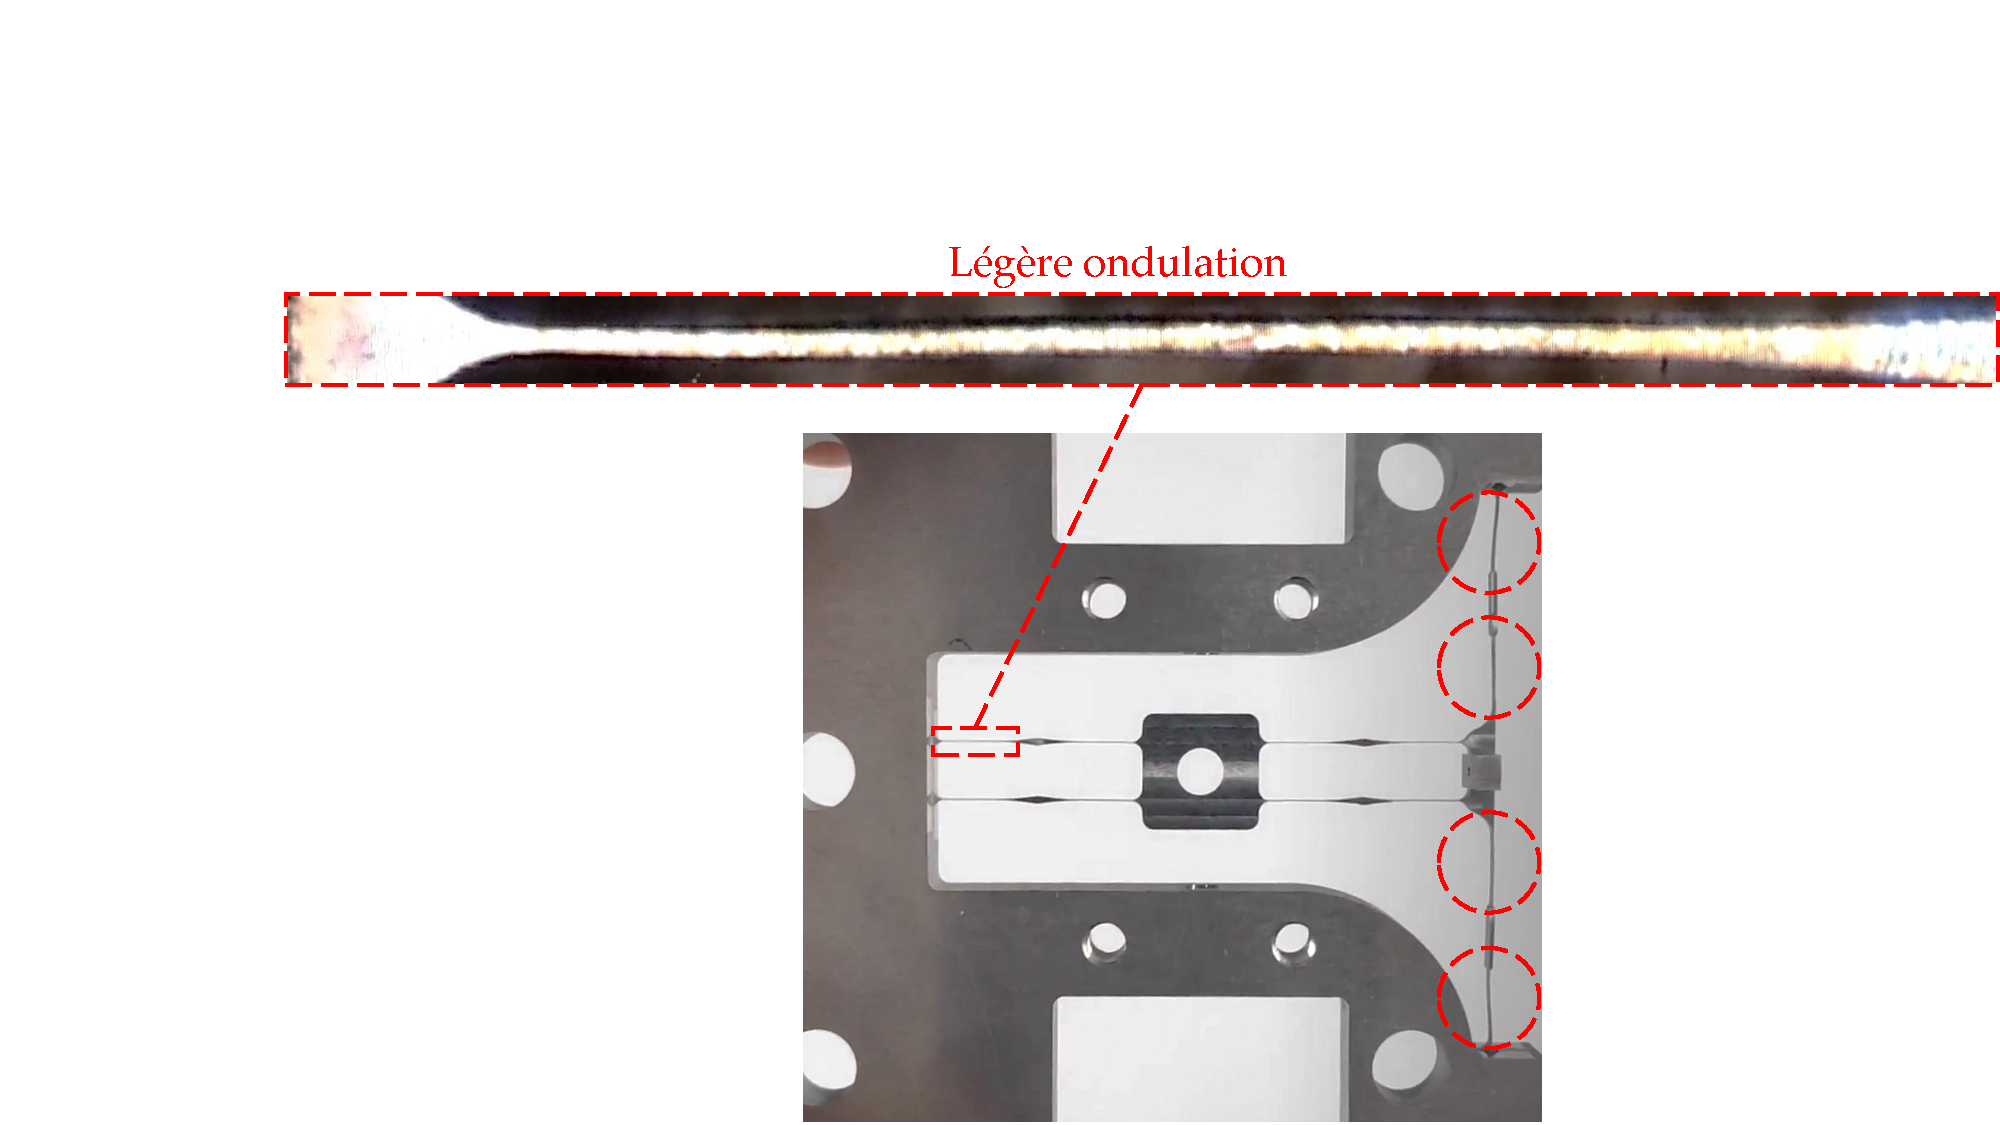
\includegraphics[trim={4.5cm 0cm 0cm 4cm},clip, width=0.9\textwidth]{../Chap3/Figure/BDT_defauts_OB.pdf}
	\caption{Mise en évidence des défauts de fabrication de l'OB monobloc}
	\label{fig:BDT_defauts_OB}
\end{center}
\end{figure}
%%%%%%%%%%%		
Par ailleurs, de légères ondulations sont observées au niveau des portions des LFs qui doivent assurer les liaisons pivot souples. Cela indique que la longueur $L$ est différente de la conception et que les propriétés mécaniques de l'OB sont différentes de celles du modèle conçu. Concrètement, des lames ondulées risquent de dégrader le coefficient de coupage de l'oscillateur car les efforts de compression sur les LFs seront en partie stockés dans les déformations locales au niveau des portions ondulées. Aussi, cela induit un assouplissement des lames en traction-compression et donc, on risque d'observer expérimentalement une raideur apparente plus faible que la valeur théorique définie à partir de la raideur $K$ du GPA.

La vis micrométrique, ainsi que le retour du capteur laser, permettent le réglage du niveau de flambement, avec une tolérance de 10µm.

Tous les essais qui suivent ont été réalisés avec le GPA branché en série sur la résistance de charge $R_{ch}$. Le coefficient de couplage électromécanique du système est alors déterminé avec les niveaux de tension du GPA, ainsi que l'amortissement électrique repéré sur la position de M. Le schéma de la figure \ref{fig:BDT_acquisition} résume les éléments du circuit d'acquisition, du circuit d'extraction et leur couplage.
%%%%%%%%%%%
\begin{figure}[!htbp]
\begin{center}
    \captionsetup{justification=centering}
	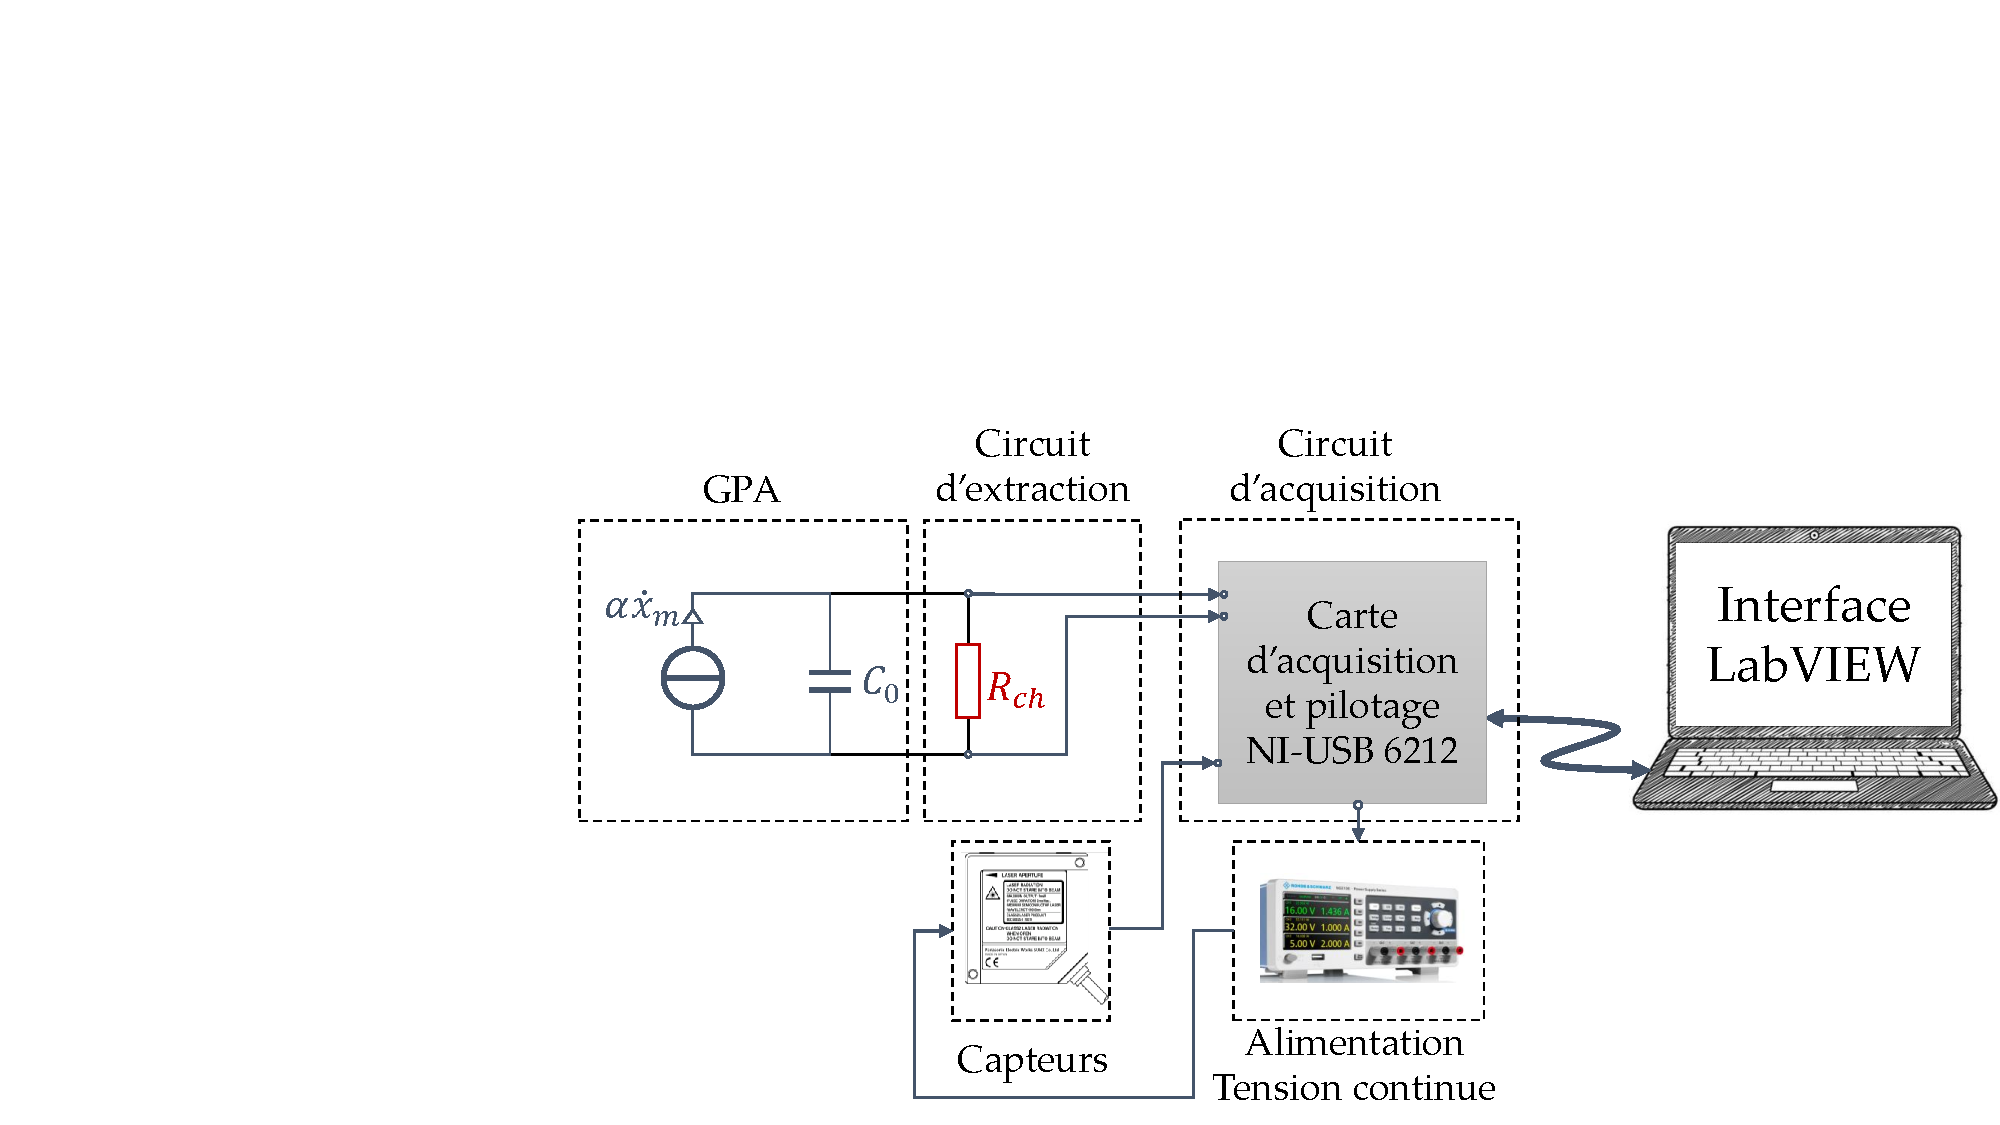
\includegraphics[trim={9.5cm 0cm 0cm 7cm},clip, width=0.7\textwidth]{../Chap3/Figure/BDT_acquisition.pdf}
	\caption{Couplage des éléments électriques du banc de test}
	\label{fig:BDT_acquisition}
\end{center}
\end{figure}
%%%%%%%%%%%		
    %/////////////////////////////////////////////
	\subsection{Corrélation modèle - essais et recalage}
    %/////////////////////////////////////////////
Le fonctionnement de l'OB dans le système global se résume au basculement alternatif de M depuis une position stable vers l'autre de façon cyclique. Le protocole d'essais consiste alors à lâcher M depuis $x=0$ pour qu'elle oscille autour d'une position stable à sa fréquence naturelle d'oscillation. On mesure alors le déplacement $x_m$, ainsi que la tension $U_p$ aux bornes de la résistance de charge. On peut donc en déduire la puissance instantanée $P_e$ traversant la résistance avec l'équation \ref{eq:P_e} et en intégrant cette dernière sur la durée d'oscillation, on peut calculer l'énergie électrique récupérée pour un basculement de M. La figure \ref{fig:BDT_correlation_simu_exp_lacher} montre alors les résultats du test de lâcher expérimental en rouge. Le modèle numérique précédemment établi est recalé en modifiant les 4 paramètres du convertisseur électromécanique : le facteur de qualité $Q$, le coefficient de couplage électromécanique $k_{sys}^2$ du système, le niveau de flambement $x_0$ et la raideur apparente $K$. Ils permettent la superposition des résultats de simulation aux données expérimentales et leur modification affecte les paramètres de l'OB de la façon qui suit :
\begin{itemize}[label=$\circ$]
	\item $Q$ est proportionnel à $x_m$ (éq. \ref{eq:w0_Q}).
	\item $k_{sys}^2$ est proportionnel à $U_p$ et inversement proportionnel à $x_m$ (éq. \ref{eq:OB-GPA_linear}).
	\item $x_0$ est proportionnel à la fréquence d'oscillation $f_0$ de M et donne la position finale de $x_m$ (éq. \ref{eq:w0_Q} et \ref{eq:x0}).
	\item $K$ est proportionnel à la fréquence d'oscillation $f_0$ de M (éq. \ref{eq:w0_Q}).
\end{itemize}

Les valeurs des paramètres ainsi recalés et celles des paramètres du modèle de pré-dimensionnement établi dans le chapitre précédent, sont présentées dans le tableau \ref{tab:parametres_lacher_free} qui met en évidence les écarts relatifs respectifs à chacun d'eux.
%%%%%%%%%%%
\begin{figure}[!ht]
\begin{center}
    \captionsetup{justification=centering}
	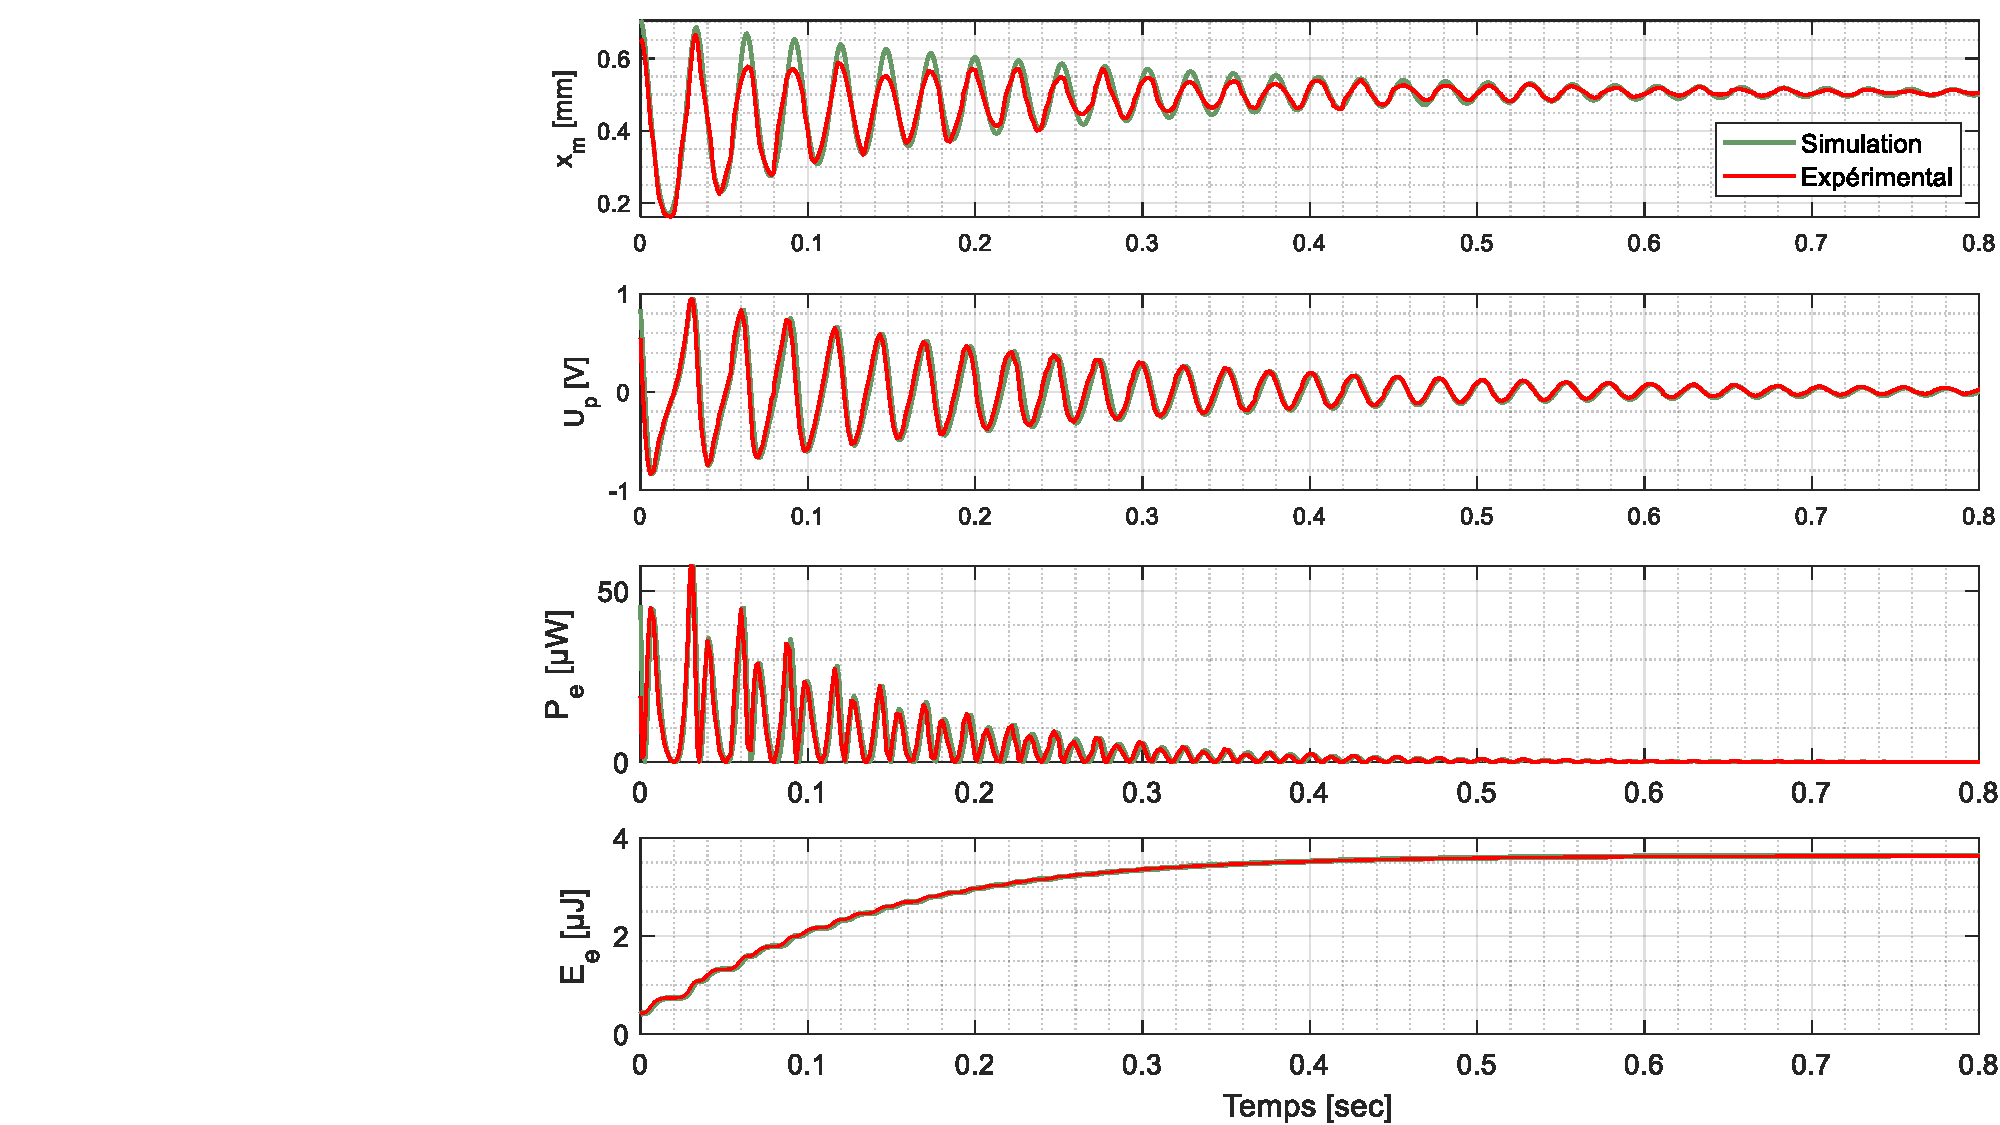
\includegraphics[trim={9cm 0cm 0cm 0cm},clip, width=\textwidth]{../Chap3/Figure/BDT_correlation_simu_exp_lacher.pdf}
	\caption{Position de M, tension du GPA, puissance dissipée dans la résistance de charge et énergie dissipée dans la résistance de charge en fonction du temps}
	\label{fig:BDT_correlation_simu_exp_lacher}
\end{center}
\end{figure}
%%%%%%%%%%%	

Les évolutions des grandeurs semblent conformes entre les données expérimentales et le modèle numérique. Cependant, des irrégularités sont notables sur la position expérimentale de M, en comparaison des données de tension du GPA. Ce phénomène n'est pas prédit par le modèle numérique. Il se peut, en effet, que la déformation locale induite sur les LFs lors de la manipulation du prototype, favorise un mode de vibration secondaire dans un plan qui est différent du plan $(zx)$. Cela peut alors influencer le déplacement de M dans le plan de mesure considéré. Une autre explication peut être l'incertitude de mesure sur $x_m$. En effet, le plan à \ang{45} servant à mesurer le déplacement de M, possède un état de surface rugueux. Cette caractéristique est nécessaire pour qu'une partie du faisceau laser émis par le capteur soit réfléchi dans le même plan d'émission, car c'est là que se trouve aussi la cellule réceptive. En revanche, l'échelle des mesures étant de l'ordre de la dizaine de µm, il se peut qu'elles ait été impactées par l'hétérogénéité de la rugosité de la surface de réflexion.\\
La première hypothèse peut être rectifiée par des LFs plus épaisses pour améliorer la robustesse durant la fabrication et la manipulation. La précontrainte de flambement sur le GPA devra être ajustée en conséquence. En effet, des lames plus épaisses seront plus difficiles à faire flamber en compression pour assurer la bistabilité de l'oscillateur. $K_{\varphi}$ sera plus grande et, en conséquence, $m_{ch}$ pour le mode de flambement utile aussi (tab. \ref{tab:multiplicateur_de_charge_flambement}). Il faudra s'assurer que la précontrainte soit dans le seuil d'admissibilité pour le GPA utilisé (<18N pour l'APA 50XS).\\
La deuxième hypothèse pourrait être rectifiée en gardant un meilleur contrôle sur la rugosité de la surface réfléchissante, ainsi que sur sa planéité.

D'autre part, les ondulations des LFs ont induit l'assouplissement des pivots souples. Cela se traduit notamment par une raideur apparente expérimentale plus faible que ce qui est prédit dans le modèle théorique. De plus, cet assouplissement joue un rôle prépondérant dans la réduction du coefficient de couplage électromécanique expérimental comparé au modèle théorique (-66\%, tab. \ref{tab:parametres_lacher_free} ). En effet, des lames plus souples auront plus de difficultés à transférer les efforts de compression au GPA et de ce fait une partie de l'énergie potentielle de M sera stockée dans les déformations locales aux points qui auront été fragilisés par la manipulation.

On peut par ailleurs extraire le rendement de conversion de l'étage de conversion électromécanique qu'est l'ensemble OB+GPA. En supposant que le lâcher s'effectue à vitesse nulle depuis la position d'équilibre instable, la hauteur de la barrière énergétique peut alors être calculée à partir de l'énergie potentielle élastique dans l'OB par l'équation \ref{eq:Barrière de potentiel expérimental}.
\begin{equation}
		\begin{split} 
		E_{b,xp}\ =&\ \frac{K_{xp}\ {x_{0,xp}}^4}{2\ L^2} \\
		E_{b,xp}\ =&\ 11.0~\text{µJ}
		\end{split}
		\label{eq:Barrière de potentiel expérimental}
\end{equation}
%%%%%%%%%%%%%%%%%
\begin{table}[!htbp]
\centering
\rowcolors[]{2}{black!8}{}{
	\begin{tabular}{ l || c | c | c }
		\rowcolor{blue!10}
		\toprule
		          						  & \textbf{Simulation avec}  	 	& \textbf{Simulation avec}   		& \textbf{Rapport paramètres}          \\
		\rowcolor{blue!10}
		\multirow{-2}{*}{\textbf{Symbole}} & \textbf{paramètres théoriques} & \textbf{paramètres expérimentaux} & \textbf{Expérimentaux/Théoriques} \\
		\midrule
		$Q$                       & 50.0                  & 30.0                     & - 40\%                   \\
		$f_0$                     & 47.0 Hz               & 27.9 Hz                  & - 40\%                   \\
		$x_0$                     & 0.49 mm               & 0.50 mm                  & + 2\%                    \\
		$K$                       & 2.56e5 N/m            & 0.85e5 N/m               & - 66\%                   \\
		${k^2_{sys}}$              & 8.72 \%               & 1.25 \%                  & - 73\%                   \\
		$\eta_{ob}$               & 79 \%                 & 12.9 \%                  & - 84\%                   \\
		\bottomrule
	\end{tabular}}
\caption{Valeur des paramètres de l'OB issus du test de lâcher expérimental, comparés aux valeurs théoriques}
\label{tab:parametres_lacher_free}
\end{table} 
%%%%%%%%%%%%%%%%%%%%%  

Le rendement expérimental $\eta _{exp}$ de l'étage de conversion électromécanique est alors défini, à travers l'équation \ref{eq:Barrière de potentiel expérimental}, comme le rapport de l'énergie électrique générée lors des oscillations par l'énergie disponible dans l'OB avant le lâcher. Ce dernier est directement lié au produit $k^2_{sys}Q$.
\begin{equation}
		\begin{split} 
		\eta _{exp}\ =&\ \frac{E_{e,xp}}{E_{b,xp}} = \dfrac{3.6}{27.7} \\
		\eta _{exp}\ \approx &\ 12.9\text{\%} \\
		\end{split}
		\label{eq:Barrière de potentiel expérimental}
\end{equation}

Le rendement théorique global du système a été estimé à $\eta _g=67.1\%$ dans le chapitre précédent suite au dimensionnement préliminaire du système (tab. \ref{tab:parametres électromécaniques}). On peut par ailleurs isoler seulement le rendement théorique du convertisseur électromécanique qui vaut alors $\eta _{ob}=79\%$. Le prototype assemblé semble avoir un rendement de conversion $84\%$ plus faible que ce que prédit la théorie. Cet écart peut être causé par deux principaux facteurs:
\begin{itemize}[label=$\circ$]
	\item Les ondulations des LGs qui induisent des une résistance en compression réduite et, par extension, une transmission des efforts au GPA réduits. La conséquence est un baisse de $Q$ et une baisse de ${k^2_{sys}}$.
	\item Les encastrements expérimentaux moins bons que ceux du modèle idéal, induisant une moins bonne transmission des efforts mécaniques au GPA. La conséquence directe est une baisse de $Q$.
\end{itemize}

Le comportement dynamique du prototype expérimental est néanmoins fidèle au modèle théorique avec un recalage des paramètres prenant en compte les dégradations induites par la fabrication et la manipulation du prototype.
    %/////////////////////////////////////////////
	\subsection{Conclusion}
    %/////////////////////////////////////////////
Il a été présenté dans ce chapitre la conception, la fabrication, ainsi que la caractérisation de l'étage de conversion électromécanique composé de l'OB et du GPA.

On a notamment vu le cahier des charges et la méthode de dimensionnement des LFs et des LGs de l'OB monobloc. Cela a été réalisé en accord avec les contraintes liées au contexte applicatif et établies dans le chapitre précédent.

Les essais expérimentaux nous ont permis de valider le comportement du convertisseur électromécanique simulé dans le chapitre précédent. En nous servant des données expérimentales, nous avons recalé les différents paramètres de l'oscillateur. Ces-derniers sont listés dans le tableau \ref{tab:parametres_lacher_free}.

Le rendement du convertisseur électromécanique fabriqué est d'environ $13\%$. Il est $84\%$ plus faible que ce que prédit la théorie et cette baisse peut être le résultat de plusieurs facteurs qui ont été identifiés. En considérant le recul sur le premier prototype, on peut donc prétendre à des améliorations sur une deuxième itération qui serait une perspective à ces travaux. En effet, par souci de temps, nous concentrerons la suite de l'étude exclusivement autour de ce premier prototype.

Pour finir, les dimensionnements qui vont suivre dans les chapitres suivants vont prendre en compte l'assouplissement de l'OB. La raideur $K$ utilisée pour calculer les paramètres statiques lors de l'intégration de la raideur $K_{VH}$ dans le modèle système sera celle identifiée expérimentalement dans le tableau \ref{tab:parametres_lacher_free}, soit $K=$84500N/m.

    